\documentclass[11pt]{scrbook}
\usepackage[utf8]{inputenc}
\usepackage[T1]{fontenc}

%% Formula typesetting, packages, etc
\usepackage{amsmath,amssymb,amsthm}
\usepackage{graphicx}
\usepackage{graphics}
\usepackage{xypic}
\usepackage[bookmarks=false]{hyperref} % Better Bibtex url entries with hyperlinks.
\usepackage[hyphenbreaks]{breakurl}
\usepackage{multirow}
\usepackage{multicol}
\usepackage{epigraph}
\usepackage[algoruled,vlined,linesnumberedhidden,norelsize]{algorithm2e} % For Algorithm boxes

% \usepackage[cc]{titlepic}

\usepackage{caption}
\usepackage{marginnote}
\usepackage[top=1in, bottom=1in, outer=1.2in, inner=1.2in, heightrounded, marginparwidth=1.5cm, marginparsep=0.5cm, includeheadfoot]{geometry}
\usepackage{wrapfig}

%% Footer
\renewcommand\pagemark{\small \emph{A Brief Introduction to Simulation -- T.~Yusun and T.~Stephen} \hfill \thepage}

\setlength{\parskip}{8pt}
\setlength{\parindent}{0pt}

\usepackage{enumerate}
\usepackage[shortlabels]{enumitem}
\usepackage{subcaption}

%% Remove blank page before each chapter
\usepackage{etoolbox}
\makeatletter
\patchcmd{\scr@startchapter}{\if@openright\cleardoublepage\else\clearpage\fi}{}{}{}
\makeatother

% Declaration styles
\newtheorem{mylemma}{Lemma}[chapter]
\newtheorem{mytheorem}{Theorem}[chapter]
\newtheorem{myconjecture}{Conjecture}[chapter]

\theoremstyle{definition}
\newtheorem{myexample}{Example}[chapter]
\newtheorem{mydefinition}{Definition}[chapter]

% New commands
\newcommand{\comb}[2]{{{#1} \choose {#2}}}
\newcommand{\scr}[1]{\mathcal{#1}}
\newcommand{\N}{\mathcal{N}}
\newcommand{\F}{\mathcal{F}}
\newcommand{\Z}{\mathbb{Z}}
\newcommand{\R}{\mathbb{R}}
\newcommand{\Q}{\mathbb{Q}}
\newcommand{\C}{\mathcal{C}}
\newcommand{\V}{\mathcal{V}}
\newcommand{\AC}{\psmat{A & 0 \cr 0 & C}}
\newcommand{\ACp}{\pmat{A & 0 \cr 0 & C}}
\newcommand{\zero}{\textbf 0}
\newcommand{\vz}{\textbf z}
\newcommand{\vb}{\textbf b}
\newcommand{\vy}{\textbf y}
\newcommand{\vx}{\textbf x}
\newcommand{\vu}{\textbf u}
\newcommand{\vv}{\textbf v}
\DeclareMathOperator{\vol}{vol}
\DeclareMathOperator{\area}{area}
\DeclareMathOperator{\intr}{int}
\DeclareMathOperator{\rank}{rank}
\DeclareMathOperator{\supp}{supp}
\newcommand{\norm}[1]{\lVert #1 \rVert}
\DeclareMathOperator{\diam}{diam}
\newenvironment{psmallmatrix}
  {\left(\begin{smallmatrix}}
  {\end{smallmatrix}\right)}
\newcommand{\mat}[1]{\begin{matrix} #1 \end{matrix}}
\newcommand{\pmat}[1]{\begin{pmatrix} #1 \end{pmatrix}}
\newcommand{\psmat}[1]{\begin{psmallmatrix} #1 \end{psmallmatrix}}

% For card suits
\DeclareSymbolFont{extraup}{U}{zavm}{m}{n}
\DeclareMathSymbol{\varheart}{\mathalpha}{extraup}{86}
\DeclareMathSymbol{\vardiamond}{\mathalpha}{extraup}{87}

% For image credits
\usepackage{xcolor}
\usepackage[absolute,overlay]{textpos} %% Place text at a location.
\newenvironment{imcredit}[2]{%
  \begin{textblock*}{\textwidth}(#1,#2)
      \tiny\bgroup\color{red!50!black}}{\egroup\end{textblock*}}

%% FRONT MATTER
\subject{\texttt{Open Optimization} Course Notes}
\title{A Brief Introduction to Simulation}
\subtitle{(Work in Progress)}
\date{Version 0.0 (January 2020)}
\author{\textbf{Timothy Yusun} \\ Department of Mathematical and Computational Sciences \\ University of Toronto Mississauga \and 
\textbf{Tamon Stephen} \\ Department of Mathematics \\ Simon Fraser University}
\publishers{ ~ \\ ~ \\ ~ 
\includegraphics[width=\linewidth]{front-matter/logo-open-optimization-oer-wide} \\ ~ \\
Copyright 2020 by Timothy Yusun and Tamon Stephen. \\ ~ \\ This work is licenced under the Creative Commons Attribution-ShareAlike 4.0
 (\href{https://creativecommons.org/licenses/by-sa/4.0/}{CC BY-SA 4.0}) license. \vspace{-3cm}}


%% BEGIN DOCUMENT
\begin{document}

\maketitle
% Incorporated into frontpage.
%        \begin{center}
%          
\includegraphics[width=\linewidth]{front-matter/logo-open-optimization-oer-wide}
%        \end{center}
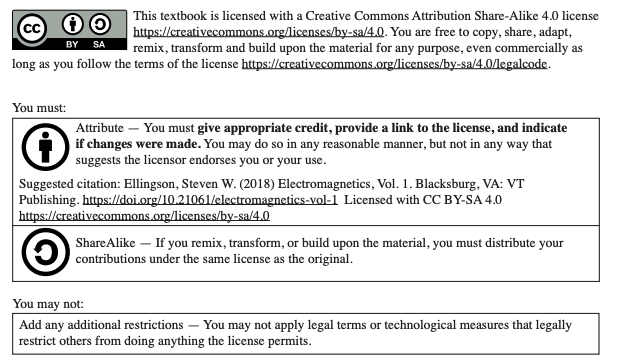
\includegraphics[scale = 0.65]{front-matter/creative-commons-statement}


This work is done in alignment with the mission of UNESCO Open Educational Resources \url{https://en.unesco.org/themes/building-knowledge-societies/oer}
\begin{center}

\includegraphics[scale = 0.1]{front-matter/Global_Open_Educational_Resources_Logo.png}\footnotemark
\end{center}
\footnotetext{\burl{https://en.wikipedia.org/wiki/Open_educational_resources\#/media/File:Global_Open_Educational_Resources_Logo.svg}}

The source code of this book is available from
\url{https://github.com/open-optimization/}

\newpage
\chapter*{Preface}
These course notes were originally written to support the course
Math 208W (Introduction to Operations Research) at Simon Fraser University
(British Columbia, Canada).
They are designed to for students with minimal mathematical background to get a hands-on
taste of Operations Research, a branch of mathematics which treats large-scale decision problems.

The focus of the course is on exploring such problems, which are too big for
analysis via pen-and-paper methods: indeed, simply collecting and managing
the data are a big part of the challenge.  The first part of the course
studies deterministic models, based on linear programming and extensions,
following Baker's \emph{Optimization Modeling with Spreadsheets}~\cite{baker2015}.  
This book suits the purpose quite well, as it assumes little in terms of prerequisites
and provides many worked examples and exercises, including data files on a supporting Website.  
The examples and exercises are written in \texttt{Microsoft Excel}, which is ubiquitous in the user
community, and a skill that Operations Researchers hoping to make an impact in practice should acquire.

For the second part of the course, we move on to non-deterministic models,
that incorporate an element of \emph{simulation}.  These notes are designed to
support this part of the course.
The notes continue in the style of Baker, with light 
prerequisites (Introductory Calculus) and extensive, \texttt{Excel}-based examples
and exercises, supported by data files.  The aim is not a rigorous presentation,
but rather an exposure to the basic ideas of simulation and an invitation to experiment.  

\vspace{4mm}
Chapter~\ref{sec1} begins the discussion with an introduction to random numbers
and how to generate them.  Chapter~\ref{sec2} then shows how a simple random
source can be used to generate different types of distributions that may be
useful in simulations.  Chapter~\ref{sec3} proceeds to use these distributions
to build some very basic simulations involving coin-flipping and random walks,
while Chapter~\ref{se:queueing} builds on this to examine simple queues and 
discrete-event simulations.  

\vspace{4mm}
There are several texts that introduce simulation.  We mention some which are
good sources for further reading, though they often require more extensive
mathematical prerequisites.  Hillier and Liebermann~\cite{hl2010} provide an
extensive introduction to Operations Research, including a chapter on
simulation.  Simulation textbooks include Bertsimas and Freund~\cite{bf2004},
Banks et al.~\cite{banks2010}, Guiasu~\cite{guiasu2009}, Law~\cite{law2015},
Leemis and Park~\cite{leemis2006} and Parlar~\cite{parlar2000}.

\vspace{4mm}
This work was started with support from a Teaching and Learning Development Grant (TLDG)
through the Institute for the Study of Teaching and Learning in the Disciplines
(ISTLD) at Simon Fraser University.  We thank the ISTLD staff who helped with
the project, including Cheryl Amundsen and Laura D'Amico for encouragement
and discussion, and the other participants in our workshop for feedback.

We thank Ismael Martinez and the students who took Math 208W \textit{Introduction to Operations Research}
at SFU for 2017-2019 for their comments and suggestions.

\vspace{4mm}
These notes are a work in progress, and comments, corrections and suggestions are encouraged.
The authors' contact details are available on their Webpages.\footnote{\url{https://www.utm.utoronto.ca/math-cs-stats/faculty-staff/yusun-dr-timothy} and \\ 
\url{http://people.math.sfu.ca/~tamon/}.}

\thispagestyle{plain} %% Or odd "Contents" header pops up.


\newpage
\tableofcontents


\newpage

\chapter{Randomness and Random Numbers}\label{sec1}
\setlength{\epigraphwidth}{3in}
\epigraph{The generation of random numbers is too important to be left to chance.}{Robert R. Coveyou \\ Oak Ridge National Laboratory, 1969.}

Randomness is \underline{unpredictability}, or \underline{a lack of any discernible pattern}.

Consider the experiment of flipping a coin -- there are two possible outcomes, heads or tails.
This is a \emph{random experiment}, since we cannot predict the outcome.
Moreover a coin flip is not reproducible as an individual event; however it is still possible to understand the relative frequencies of the possible outcomes by repeating this experiment multiple times.
Flipping a fair coin 1000 times, for instance, will give roughly 500 heads and 500 tails.

With a view towards modelling these random experiments, first we discuss random numbers and how to generate them.

\textbf{Question}: Would you characterize the sequence of digits of $\pi$ as \emph{random}?
$$\pi = 3.14159265358979323846\cdots$$
This sequence looks random, in the sense that these digits do not seem to follow any prescribed pattern.
On the other hand, $\pi$ is a fixed number, and any digit of this sequence can be calculated given sufficient resources.
We call such a sequence \emph{pseudorandom}.
This means that the process that outputs digits of $\pi$ in sequence \emph{appears random}, statistically speaking, while being completely deterministic.

In fact, the following process can be used as a [bad] algorithm for generating random numbers from the set $\{0, 1, \ldots, 9\}$:

\begin{algorithm}
\textbf{initialize} $i$ a non-negative integer\;
\textbf{function} rand(): \\
\qquad 	$i \leftarrow i + 1$\;
\qquad	\textbf{return} $i$th digit of $\pi$ \;
\caption{A simple random number generator}
\label{alg:pi}
\end{algorithm}

One nice property of this is algorithm is that as long as we know the initial index $i$, we can repeat exactly the sequence of digits it outputs.
This is called the \emph{seed} of the generator.
This is especially useful for running computer simulations, as sometimes we would like to reproduce results of simulating a random process.
Note that we would not actually use Algorithm~\ref{alg:pi} in a simulation, due to a large part in the computational effort required to compute digits of $\pi$.
Moreover, patterns have been found in its digits\footnote{See \url{http://mathworld.wolfram.com/PiDigits.html}}.
Another simple example is Algorithm~\ref{alg:lin_cong}.


\begin{algorithm}
\textbf{initialize} integers $a$, $m$, $c$ appropriately selected, a seed $x_0$, $i = 0$ \;
\textbf{function} rand(): \\
\qquad $i \leftarrow i + 1$ \;
\qquad $x_{i} = (ax_{i-1} + c)$ \ (mod $m$) \;
\qquad	\textbf{return} $x_i$ \;
\caption{The Linear Congruential Method}
\label{alg:lin_cong}
\end{algorithm}


The $\mod$ here is the \emph{modulo operation} -- it computes the remainder when $(ax_{i-1} + c)$ is divided by $m$.
This means each $x_i$ will be in the set $\{0,1,2,\ldots,m-1\}$.
As in Algorithm~\ref{alg:pi}, Algorithm~\ref{alg:lin_cong} is very easy to replicate, in this case by simply knowing the parameters $a$, $m$, $c$, and the seed $x_0$.

There are certain conditions that these parameters have to satisfy in order to make this algorithm viable.
One desirable property of the produced sequence is a long period, that is, that the algorithm goes through as many values from the set $\{0,1,2,\ldots,m-1\}$ as possible.
For instance, if $c = 0$ and $m$ is prime, the algorithm generates the longest possible period with length $m - 1$ for many values of $a$.\footnote{This holds if $a$ is chosen so that the smallest integer $k$ such that $a^k - 1$ is divisible by $m$ is $k = m - 1$. Such an $a$ is called a \emph{primitive root modulo $m$} -- see \cite{law2015}.}
This algorithm can be modified to output real numbers in $(0,1)$, by dividing the outputs by $m$. 

\begin{myexample} [The Linear Congruential Method]

	Using $a = 6$, $m = 11$, $c = 0$, and $x_0 = 1$, we get the sequence $1, 6, 3, 7, 9, 10, 5, 8, 4, 2,  \ldots$ which goes through all values in $\{1, 2, \ldots, 10\}$ before repeating.

	If we use the same parameters but with $m = 10$ instead, we get $1, 6, 6, 6, \ldots$, reminding us that we need to pay attention to $m$, $a$, and $c$.
\end{myexample}

This example illustrates the operations performed.
Observe that as in Algorithm~\ref{alg:pi}, the output of this algorithm is completely deterministic.
It also becomes more predictable the more numbers you've generated, since you do not repeat $x_i$'s before the period ends (and then after that, the same sequence is produced repeatedly).

In practice however, $m$ is chosen to be very large, and if the other parameters are chosen correctly, the sequence produced will look no different than a random sequence (in the sense that it passes known statistical tests that check for this property).

There are more sophisticated algorithms for random number generation, based on similar ideas to Algorithm~\ref{alg:lin_cong}. 
One popular one is called the \emph{Mersenne Twister}, and which is used by most computational software, including MATLAB, Excel, C++, and others.
For running simulations on a computer, the primary concern in this course is knowing how to use a computer to generate random numbers (although it is helpful understanding how it is done in the background).

\section{Generating Random Numbers in Excel}
In Microsoft Excel, the \texttt{=RAND()} command outputs a random real number\footnote{In computing, real numbers are represented as \emph{floating point numbers} \\ -- see \url{https://en.wikipedia.org/wiki/Floating_point}.} in the interval $[0,1)$.
Whenever the worksheet is re-calculated (by editing a cell, for example), a new real number is returned in this interval.

This function can be in turn used to generate a random real number in any interval $[a,b)$, using the formula \texttt{= a + (b - a)*RAND()}.
Intuitively, this transformation computes the number in the interval $[a,b)$ that is \texttt{RAND()} fraction of the way from $a$ to $b$.

\begin{figure}[htbp]
	\centering
	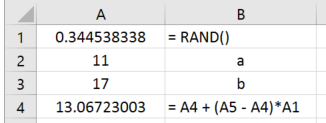
\includegraphics[width=0.45\textwidth]{fig/1_excel_rand.png}
	\caption{Computing random real numbers in Excel}
	\label{fig:excel_rand}
\end{figure}

Note that this process is \emph{not} reproducible; once the worksheet is refreshed, each \texttt{RAND()} call is reset, and the old values cannot be retrieved.
There are two ways of fixing the values generated -- one is to copy and paste these in a separate worksheet; another way is to press F9 after entering the formula instead of Enter.
This makes it so that recalculations are not done when the worksheet is refreshed, and the formula in the cell is overwritten by the computed values.

The type of randomness we discuss in this section is called \emph{uniform}, since numbers from the set under consideration are all \emph{equally likely} to be generated.
We also call this a \emph{uniform distribution} of numbers.

One way of visualizing the random numbers we are generating is by using \emph{histograms}, which are graphs with rectangles or bars representing the frequency of each range of values.
In Figure~\ref{fig:histogram} we show the result of generating 100 real numbers using \texttt{RAND()}, then grouping results into `buckets' $[0,0.1), [0.1,0.2), \ldots, [0.9,1)$. 

\begin{figure}[htbp]
	\centering
	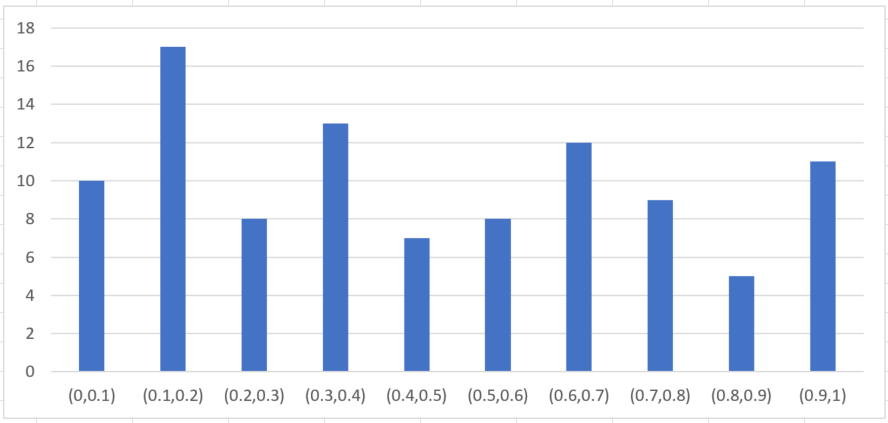
\includegraphics[width=0.6\textwidth]{fig/1_histogram.png}
	\caption{A histogram of one hundred \texttt{RAND()} outputs in Excel \label{fig:histogram}}
\end{figure}

Note that there are 17 numbers in $[0.1,0.2)$ while only 5 in $[0.8,0.9)$.
This is not unusual -- what we would expect the average to be when repeating an experiment multiple times does not necessarily reveal itself in only a few trials.
Observe that the histogram in Figure~\ref{fig:histogram1000}, where we generate a thousand real numbers using \texttt{RAND()}, looks more `evened out.'

\begin{figure}[htbp]
	\centering
	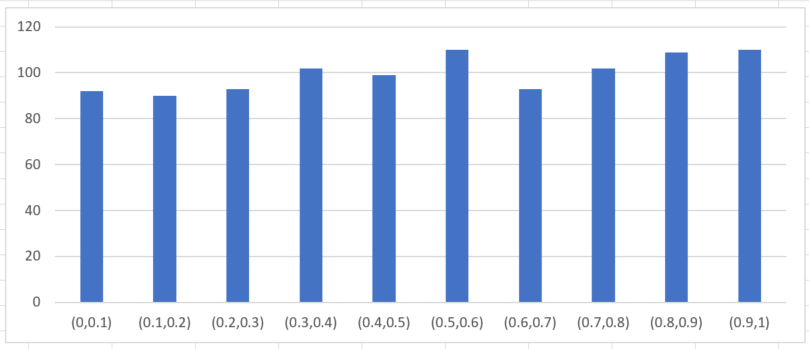
\includegraphics[width=0.6\textwidth]{fig/1_histogram_1000.png}
	\caption{A histogram of one thousand \texttt{RAND()} outputs in Excel \label{fig:histogram1000}}
\end{figure}


In the next section, we will introduce other types of distributions, where some outcomes are more likely than others.
From this point we will use the term \emph{random number} to describe a random real number from $[0,1)$, and the term \emph{random variable} to describe an output that may be generated from any
general probability distribution. 


\begin{center}
	\textbf{EXERCISES}
\end{center}

\begin{enumerate}[label={1.\arabic*},leftmargin=1cm]
	\item \textbf{Explore.} Write a sequence of H's and T's to describe what you think will happen if you flip a coin twenty times. How about fifty? Then actually perform the experiments, and compare the two results. What observations can you make?
	\item An urn contains ten balls - three blue, two green, and five red. \label{exer:1_urn}
		\begin{enumerate}[(a)]
			\item If you pick a ball at random, what are the chances that the ball is blue? red? 
			\item If you pick two balls in succession (without putting back the first ball), what are the chances that the two balls are green?
		\end{enumerate}
	\item What are the chances that you roll a die twice and you never see the number 1? How about three times?
	\item When we take $c = 0$ in Algorithm~\ref{alg:lin_cong}, it is known as the \emph{Multiplicative Congruence Method}, also called the \emph{Lehmer random number generator} after the mathematician D.~H.~Lehmer. A classical choice for its parameters is $m = 2^{31} - 1 = 2147483647$ and $a = 7^5 = 16807$, and this generator has the special name \texttt{MINSTD}. Using Excel, generate the first ten terms of \texttt{MINSTD} when the initial seed is your SFU student ID number. (Divide each term by $m$ so that each output lies in $[0,1)$.) \label{exer:1_Lehmer}
	\item Write a formula in Excel to generate a number uniformly from the following sets:
		\begin{enumerate}[(a)]
			\item The interval $[0, 100)$.
			\item The interval $(-20, -15]$.
			\item The set of integers in the interval $[-20,-15]$.
		\end{enumerate}
	\item Write a formula in Excel that simulates the process of picking a ball at random from the urn in Exercise~\ref{exer:1_urn}
	\item \textbf{Explore.} Replicate the process used in Figure~\ref{fig:histogram} and Figure~\ref{fig:histogram1000} but using different bucket sizes - $0.2$ and $0.05$. That is, generate one hundred, then one thousand random numbers from $[0,1)$, and then aggregate the results using (a) 5 buckets of equal length; (b) 20 buckets of equal length. What do you think the effect of changing the bucket size will be? Compare with the results of your experiment.
	\item Explain the following \texttt{xkcd} comic:
		\begin{figure}[htbp]
			\centering
			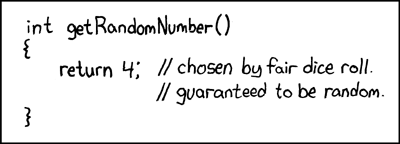
\includegraphics[width=0.5\textwidth]{fig/1_xkcd_random_number.png}
			\captionsetup{labelformat=empty}
			\label{fig:xkcd_random}
			\caption{Source: \texttt{https://xkcd.com/221/}}
		\end{figure}
\end{enumerate}




\newpage

\chapter{Probability Distributions}\label{sec2}
\setlength{\epigraphwidth}{3in}
\epigraph{One sees... that the theory of probabilities is basically just common sense reduced to calculus.}{Pierre-Simon Laplace \\ \emph{Philosophical Essay on Probabilities}, 1814}

\section{The Discrete Uniform Distribution, PDFs and CDFs}\label{sec2:discreteuni}

In this section we consider probability distributions and how to sample them on a computer.\footnote{For further reading on probability distributions, see \cite{larsenmarx2004}.}
The \textbf{probability} of an event is a measure of how likely that event will occur, it can be understood as the ratio of the number of ways it can occur to the entire space of possible outcomes.
\textbf{Probability distributions} contain information about the probabilities of different possible outcomes in an experiment.
In the next example we define two important probability functions.

\begin{myexample}\label{2_dice_example}
Consider the experiment of rolling a fair six-sided die with the numbers 1 to 6 on its faces.
Each face has an equal chance of coming up when the die is rolled -- so the probability that we get the number 1 (e.g.) is $\frac{1}{6}$.
Using $X$ to denote the random variable representing the outcome of this experiment, we can state this as $P(X = 1) = \frac{1}{6}$. Similarly, $P(X = 2) = \frac{1}{6} = P(X = 3) = \cdots$.

\begin{figure}[htbp]
	\centering
	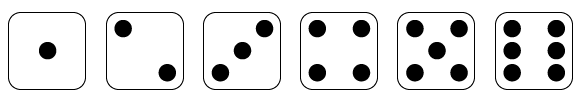
\includegraphics[width=0.6\textwidth]{fig/2_dice_example.png}
	\caption{Each outcome has equal probability $= \frac{1}{6}$. \label{fig:2_dice_example}}
\end{figure}


The probability distribution for $X$ assigns a probability of $\frac{1}{6}$ to each of the six possible outcomes -- this is the \emph{uniform distribution} from Section~\ref{sec1} applied to the integers $\{1,2,\ldots,6\}$. 
We can capture this information concisely using a \textbf{probability density function}, or a \textbf{pdf}.
This is a function $f(k)$ that takes as input the outcome $k$, and outputs the probability that $X = k$.
That is, the pdf for the random variable $X$ is \[ f(k) = P(X = k) = \left\{ \begin{matrix} \frac{1}{6}, & k = 1,2,\ldots, 6 \cr 0, & \text{ otherwise.} \end{matrix} \right. \]


Recall from Section~\ref{sec1} that we call this a uniform distribution, since each outcome is equally likely.
In particular, $X$ is said to have a \textbf{discrete uniform distribution}, since there are only a finite number of possible outcomes.

We also define the \textbf{cumulative distribution function} of a random variable, also called its \textbf{cdf}.
As the name suggests, this function $g(k)$ takes as input an outcome $k$, and outputs the probability that $X \leq k$; that is, $g(k) = P(X \leq k)$.
For this example, the cdf of $X$ is \[ g(k) = P(X \leq k) = \frac{\lfloor k \rfloor}{6}, \ k = 1,2,\ldots,6. \qed \] 

\begin{figure}[htbp]
 \begin{minipage}{.5\textwidth}
        \centering
	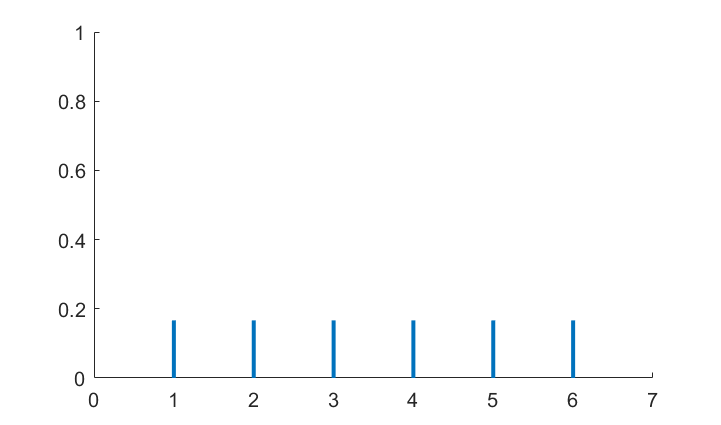
\includegraphics[width=0.9\linewidth]{fig/2_dice_pdf}
    \end{minipage}
    \begin{minipage}{0.5\textwidth}
        \centering
	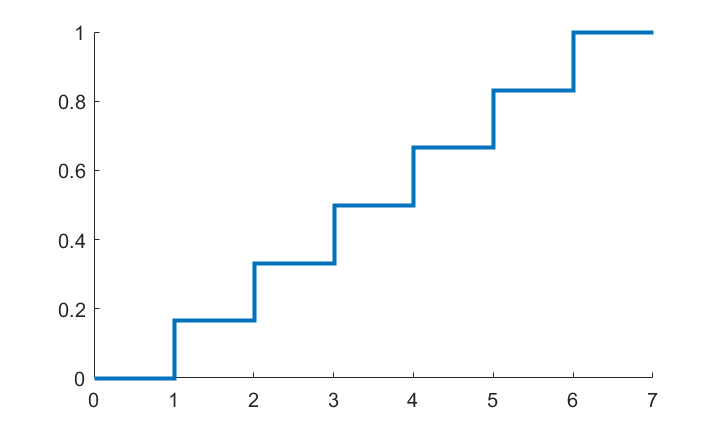
\includegraphics[width=0.9\linewidth]{fig/2_dice_cdf}
    \end{minipage}	
    \caption{The pdf (L) and cdf (R) of $X$\label{fig:2_dice_pdf}}
\end{figure}


\end{myexample}

In general, given a finite set of outcomes $S = \{a,a + 1,\ldots,b\}$, with $n = |S| = b-a+1$, the discrete uniform distribution over this set has pdf \[ f(k) = \left\{ \begin{matrix} \frac{1}{n}, & k \in S \cr 0, & \text{ otherwise.} \end{matrix} \right.\]
while its cdf is \[ g(k) = \left\{ \begin{matrix} 0, & k < a \cr \lfloor \frac{k - a + 1}{b - a + 1} \rfloor, & a \leq k \leq b \cr 1, & k > b \end{matrix} \right. \]
If a random variable $X$ has such a distribution, we denote it by $X \sim U\{a,b\}$.


To sample from the discrete uniform distribution $U\{a,b\}$ in Excel, we generate a random number using \texttt{RAND()}, then we divide the interval $[0,1)$ into an subintervals of equal length.
Recall Figure~\ref{fig:histogram1000}, which illustrated a thousand \texttt{RAND()} outputs in Excel, aggregated into intervals of width $0.1$.
This is equivalent to sampling from $U\{1,10\}$ a thousand times, mapping intervals $\left[\frac{i-1}{10},\frac{i}{10}\right)$ to the integer $i$.
In Figure~\ref{fig:2_histogram_uniform} we show the results of generating 10, 100, 1000, and 10000 random integers from $\{1,2,\ldots,10\}$.

Excel has a built in function which does this transformation for you; \texttt{RANDBETWEEN($a$,$b$)} generates a uniform random integer between integers $a$ and $b$ (inclusive).

\begin{figure}[htbp]
	\centering
	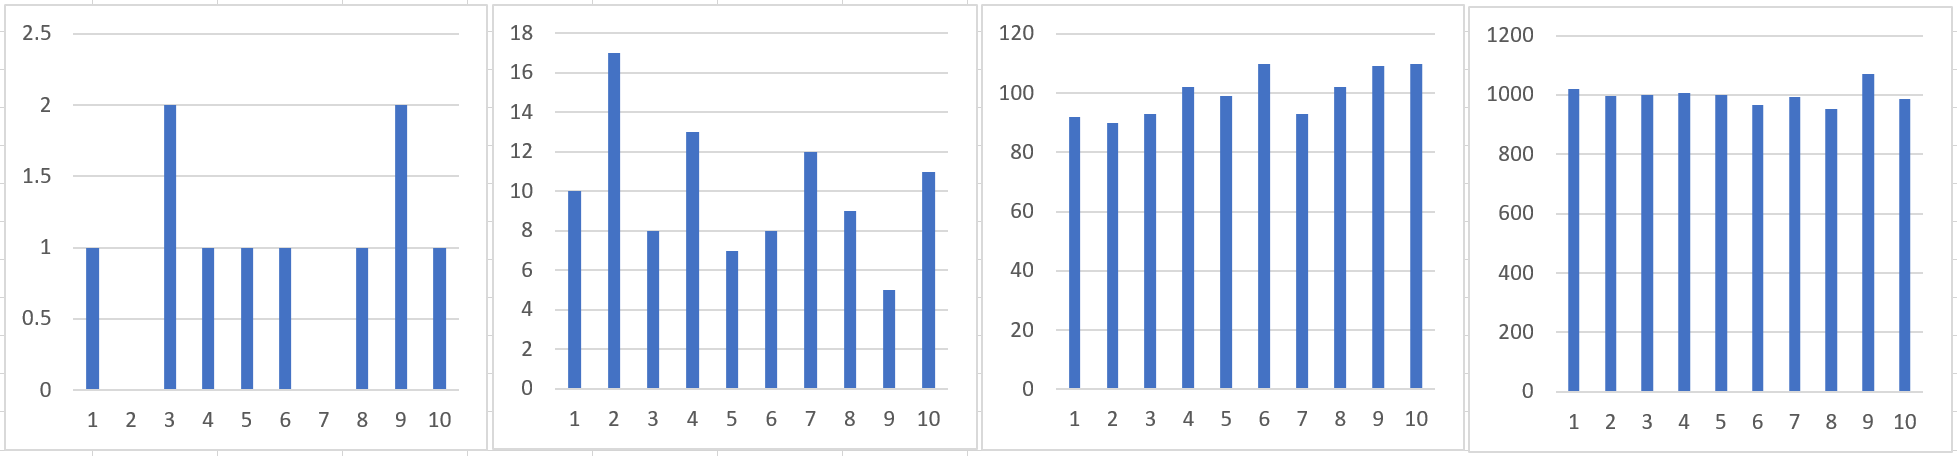
\includegraphics[width=\textwidth]{fig/2_histogram_uniform.png}
	\caption{Generating 10, 100, 1000, and 10000 values from $U\{1,10\}$ \label{fig:2_histogram_uniform}}
\end{figure}


\newpage

\section{The Bernoulli and Binomial Distributions}\label{sec2:binomial}

One of the most basic distributions is the \textbf{Bernoulli distribution}, where there are only two possibilities: \emph{success} or \emph{failure}, with a parameter $p$ describing probability of success, and a corresponding probability of $q = 1-p$ for failure.
Because there are only two possible outcomes, this is a discrete distribution.
Note that for $p = 0.5$ this is the discrete uniform distribution $U\{0,1\}$, and simulates a fair coin flip; for other values of $p$ it simulates an unfair coin flip.
We denote a Bernoulli-distributed random variable with parameter $p$ as $B(p)$.

The pdf of $B(p)$ is \[ f(k) = \left\{ \begin{matrix} 1-p, & k = 0 \cr p, & k = 1 \cr 0, & \text{ otherwise} \end{matrix} \right. \]
while its cdf is \[ g(k) = \left\{ \begin{matrix} 0, & k < 0 \cr 1-p, & 0 \leq k < 1 \cr 1, & k \geq 1 \end{matrix} \right. \]

\begin{figure}[htbp]
 \begin{minipage}{.5\textwidth}
        \centering
	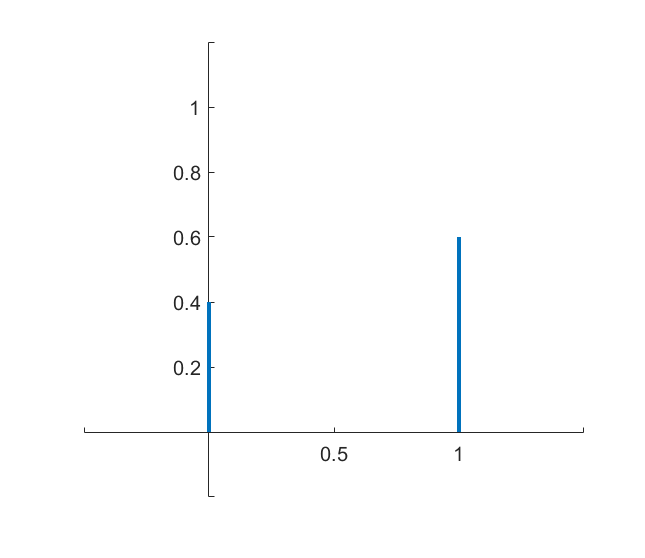
\includegraphics[width=0.9\linewidth]{fig/2_bernoulli_pdf}
    \end{minipage}
    \begin{minipage}{0.5\textwidth}
        \centering
	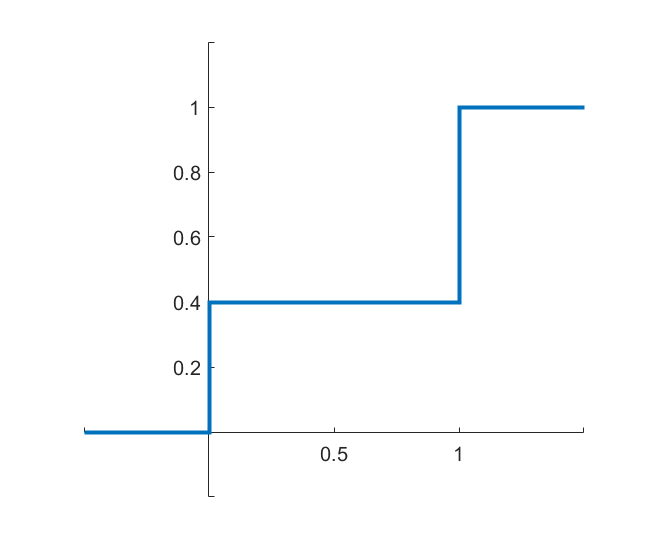
\includegraphics[width=0.9\linewidth]{fig/2_bernoulli_cdf}
    \end{minipage}	
    \caption{The pdf (L) and cdf (R) of the Bernoulli distribution with $p = 0.6$\label{fig:2_bernoulli_pdf}}
\end{figure}

To simulate this in Excel we use \texttt{RAND()} as well.
If $u$ was the result of \texttt{RAND()}, then we output $$\left\{\mat{\text{success,} & \text{if } 0 \leq u < p \cr \text{failure,} & \text{if } p \leq u < 1}\right. .$$

If we perform a Bernoulli trial multiple times, we get another distribution -- the \textbf{binomial distribution}, which counts the number of successes in $n$ independent Bernoulli trials.
Hence a binomially-distributed variable has two parameters - $p$ the probability of success for each trial, and $n$ the number of trials.
We denote this by $B(n,p)$ (so the Bernoulli distribution can also be written as $B(1,p)$).\footnote{So if $X_1, X_2, \ldots, X_n \sim B(1,p)$ independently, then $X_1 + X_2 + \cdots + X_n \sim B(n,p)$.}

\begin{myexample}
Consider the experiment of flipping two fair coins and counting the number of heads that come up.
This is a binomial random variable, with parameters $n = 2$ and $p = 0.5$.
There are three possible outcomes - zero, one, or two heads.
We can compute the probability of each outcome happening:

Ways to get zero heads: TT.

Ways to get one heads: HT or TH.

Ways to get two heads: HH.

Thus, we get the probabilities $\frac{1}{4},\frac{1}{2},\frac{1}{4}$ for each possible outcome. \qed
\end{myexample}

\begin{figure}[htbp]
 \begin{minipage}{.5\textwidth}
        \centering
	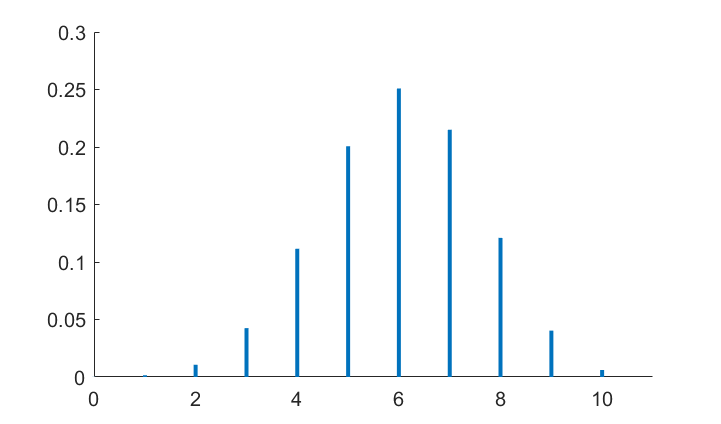
\includegraphics[width=0.9\linewidth]{fig/2_binomial_pdf}
    \end{minipage}
    \begin{minipage}{0.5\textwidth}
        \centering
	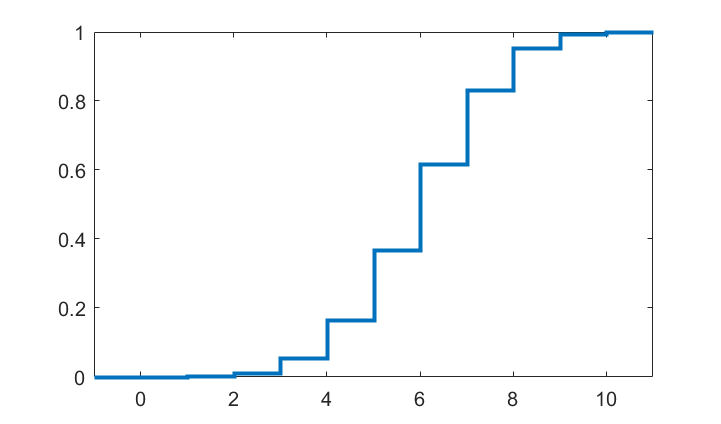
\includegraphics[width=0.9\linewidth]{fig/2_binomial_cdf}
    \end{minipage}	
    \caption{The pdf (L) and cdf (R) of the binomial distribution with $n = 10$ and $p = 0.6$\label{fig:2_binomial_pdf}}
\end{figure}



In Excel, multiple Bernoulli trials in separate cells can be used to simulate a binomial random variable by counting the number of successes.
Note in Figure~\ref{fig:excel_binomial} the use of the \texttt{IF} function -- it will output either 1 or 0 depending on whether the first condition \texttt{A3 < \$C\$1} is true or false.


\begin{figure}[htbp]
	\centering
	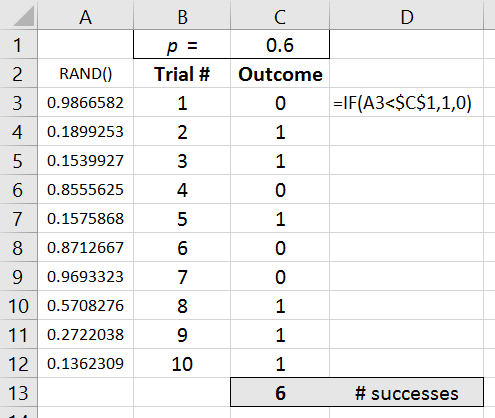
\includegraphics[width=0.35\textwidth]{fig/2_excel_binomial.png}
	\caption{Simulating multiple Bernoulli trials in Excel}
	\label{fig:excel_binomial}
\end{figure}

The exact probabilities of each outcome can be calculated analytically, and in Excel using the built-in \texttt{BINOM.DIST($x$,$n$,$p$,cumulative)}. 
This outputs the value of the pdf of $B(n,p)$ at $x$ when the argument \texttt{cumulative} is set to False. 
If \texttt{cumulative} is set to True, this function instead evaluates the cdf of $B(n,p)$ at $x$, or the probability of getting at most $x$ successes.

The function \texttt{BINOM.INV($n$,$p$,prob)} computes the inverse of \texttt{BINOM.DIST}, and can be used to generate samples from the binomial distribution.
It outputs, given the parameters $n$, $p$, and a given probability \texttt{prob}, the smallest integer for which the cumulative binomial distribution is at least \texttt{prob}.
Hence we can generate binomially-distributed variates by using \texttt{RAND()} as an input.
Figure~\ref{fig:2_excel_binominv} illustrates this process while Figure~\ref{fig:2_binomial_cdf_inv} shows the inverse of the cdf for $B(10,0.6)$.

\begin{figure}[htbp]
\centering
 \begin{minipage}{.45\textwidth}
        \centering
	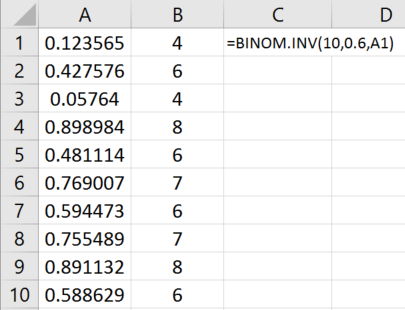
\includegraphics[width=0.9\textwidth]{fig/2_excel_binominv2.png}
	\captionsetup{font=small}
	\caption{10 outcomes from $B(10,0.6)$ \label{fig:2_excel_binominv}}
    \end{minipage}
    \begin{minipage}{0.55\textwidth}
        \centering
	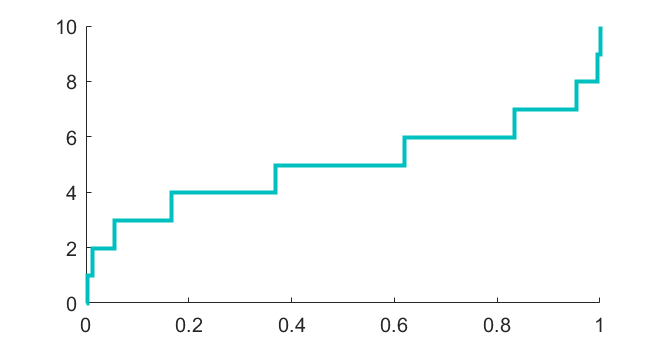
\includegraphics[width=0.95\textwidth]{fig/2_binomial_cdf_inv.png}
	\captionsetup{font=small}
	\caption{The inverse of the cdf for $B(10,0.6)$ \label{fig:2_binomial_cdf_inv}}
    \end{minipage}	
\end{figure}


In Figure~\ref{fig:2_histogram_binomial} we show the result of using Excel to generate 10, 100 and 1000 outcomes from $B(10,0.6)$.
Observe that outcomes are clustered around $6$ and that the curve has a distinct `bell' shape.
We discuss this phenomenon in Section~\ref{sec2:normal}.


\begin{figure}[htbp]
	\centering
	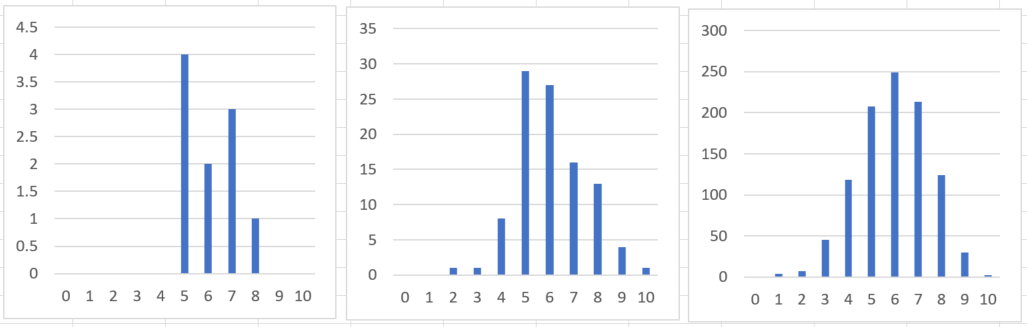
\includegraphics[width=0.75\textwidth]{fig/2_histogram_binomial.png}
	\caption{Generating 10, 100, and 1000 outcomes from $B(10,0.6)$ in Excel \label{fig:2_histogram_binomial}}
\end{figure}




\section{The Continuous Uniform Distribution, PDFs and CDFs}

We discussed in Section~\ref{sec2:discreteuni} the discrete uniform distribution $U\{a,b\}$, where each outcome in the set $\{a,a+1,a+2,\ldots,b\}$ is equally likely.

There is also a continuous version of this distribution, where the possible set of outcomes is an interval of real numbers.
Let us denote by $U(a,b)$ the continuous uniform distribution on the interval $[a,b]$.
Sampling a value $u$ from the standard continuous uniform distribution $U(0,1)$ is exactly what the \texttt{RAND()} function in Excel is designed to approximate.\footnote{Note that since the sample space is an infinite set, the probability of generating any specific value from $U(0,1)$ is 0.}
We can use $u$ to simulate the random variable $U(a,b)$, using the transformation $a + (b-a)u.$

\textbf{Question}: Do continuous random variables have probability density functions?

The answer to this question is \emph{yes}, but we will have to define them differently.
Since continuous random variables have infinitely many possible outcomes, we do not want to talk about probabilities of individual outcomes, but instead, the probability that an outcome will lie \emph{in a given interval}.

To illustrate, suppose we know that $X \sim U(0,2)$.
Then, intuitively, the probability that $X < 0.5$ should be $0.25$, which is the length of the interval $[0,0.5)$ divided by the length of the interval $[0,2)$.

So, for a continuous random variable $X$, its \textbf{probability density function} or \textbf{pdf} is a function $f(x)$, that satisfies the property that 
\begin{center}$P(a \leq X \leq b) = $ the area under the graph of $f(x)$ in between $x = a$ and $x = b$. \footnote{If you have taken integral calculus you may recognize this as the integral of $f(x)$ from $a$ to $b$: \\ $ P(a \leq x \leq b) = \int_a^b f(x) \, dx .$}\end{center}

\vspace{-0.3cm}
For example, for $U(a,b)$, its pdf is $f(x) = \left\{ \begin{matrix} \frac{1}{b-a}, & a \leq x \leq b \cr 0, & \text{ otherwise}\end{matrix} \right.$.

The \textbf{cdf} $g(x)$ of a continuous random variable is defined in the same way: \[ g(x) = P(X \leq x).\]
The cdf of $U(a,b)$ is \[ g(x) = \left\{ \begin{matrix} \frac{x-a}{b-a}, & a \leq x \leq b \cr 0, & \text{ otherwise} \end{matrix} \right. . \]

For now, do not worry about dealing with these functions themselves; what is more important is that we know how to simulate these random variables using Excel.

\begin{figure}[htbp]
 \begin{minipage}{.5\textwidth}
        \centering
	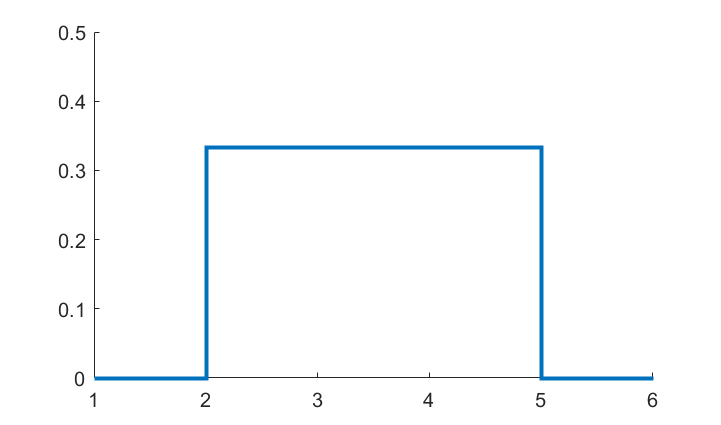
\includegraphics[width=0.9\linewidth]{fig/2_uni_pdf}
    \end{minipage}
    \begin{minipage}{0.5\textwidth}
        \centering
	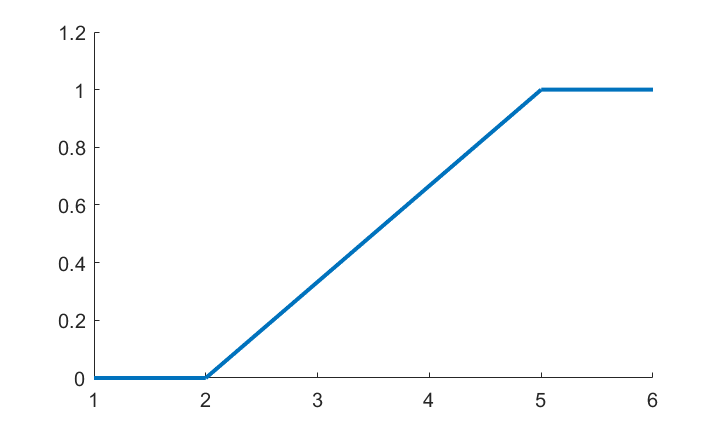
\includegraphics[width=0.9\linewidth]{fig/2_uni_cdf}
    \end{minipage}	
    \caption{The pdf (L) and cdf (R) of the continuous uniform distribution $U(2,5)$\label{fig:2_uni_pdf}}
\end{figure}

\subsection{Application: Area and Volume Computations}\label{sec2:areavolume}

One surprising application of the continuous uniform distribution is the approximation of quantities that are not random at all: areas, volumes, and their higher-dimensional analogues.
For instance, suppose we want to calculate the area of the quarter-circle in Figure~\ref{fig:4_quartercircle}.

\begin{wrapfigure}{r}{5.5cm}
	\centering
	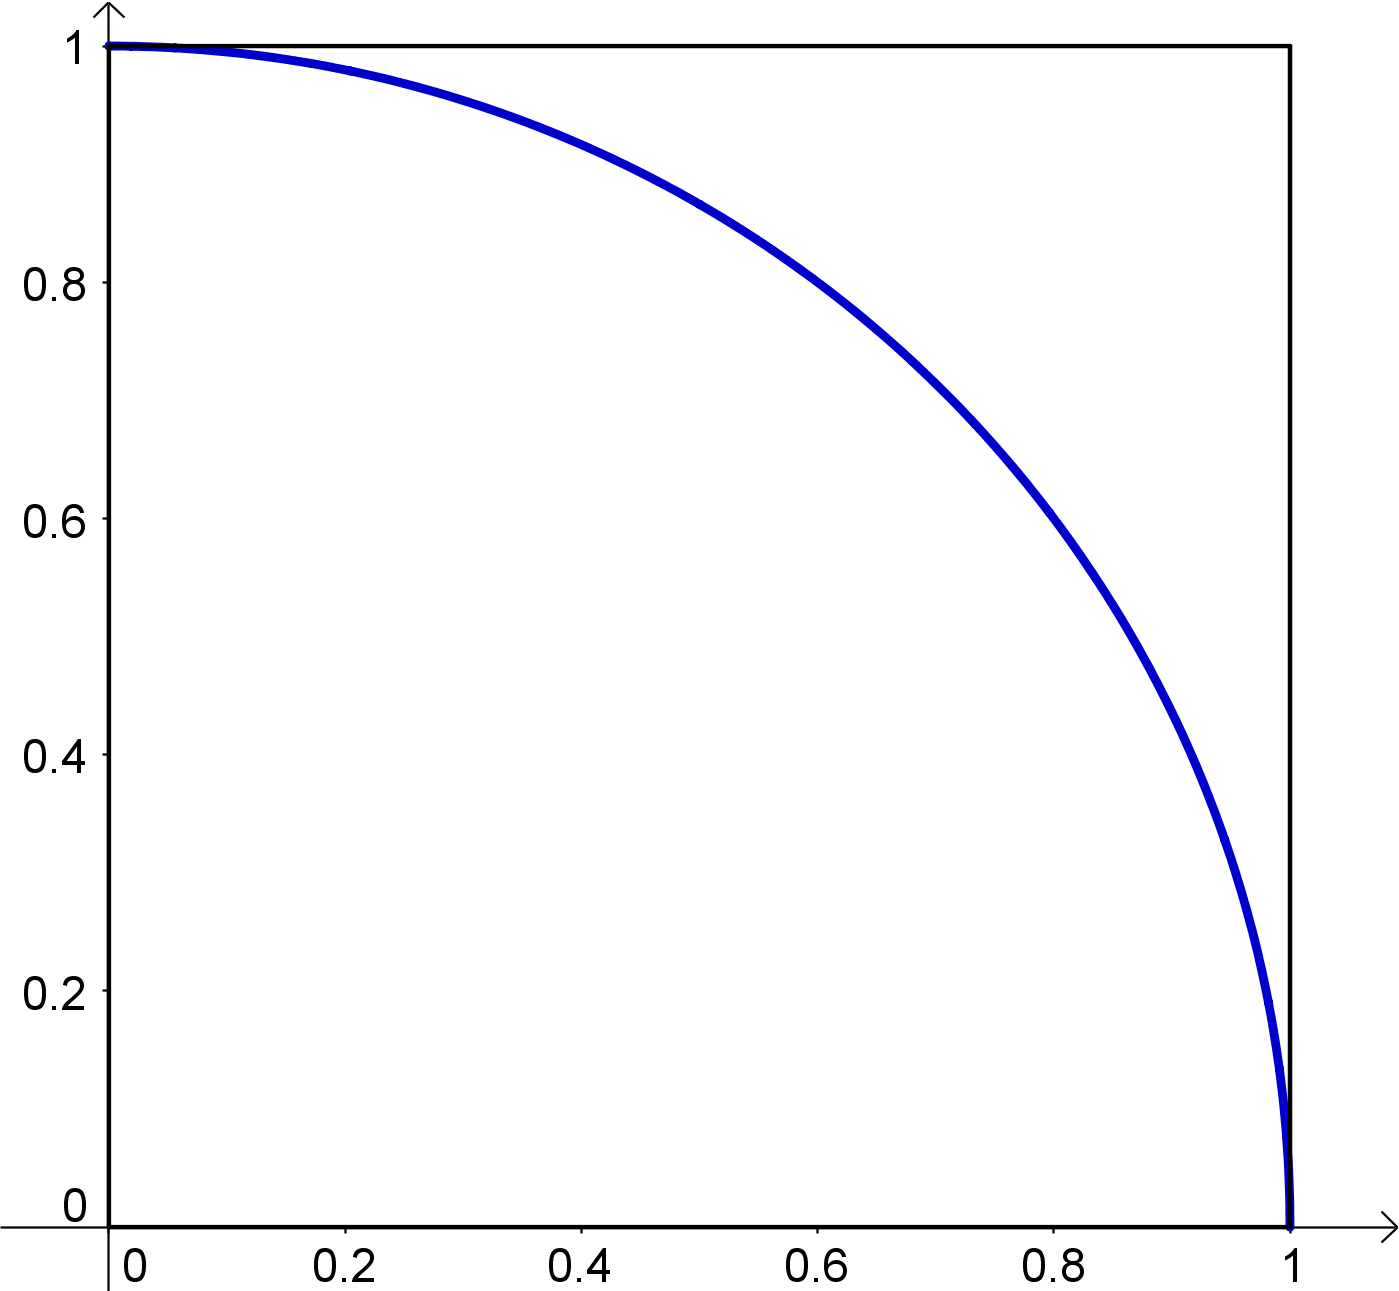
\includegraphics[width=4.8cm]{fig/4_quartercircle.png}
	\caption{\label{fig:4_quartercircle}}
\end{wrapfigure}

We know from grade-school geometry that this area is equal to $\frac{\pi}{4}$.
We can also approximate this area as follows.
We generate points at random inside the unit square, count the number of points inside the given region, and divide this by the total number of points generated.
Since the unit square has area 1, the result will be an approximation of the area of the given region.

\iffalse

\begin{figure}[htbp]
	\centering
	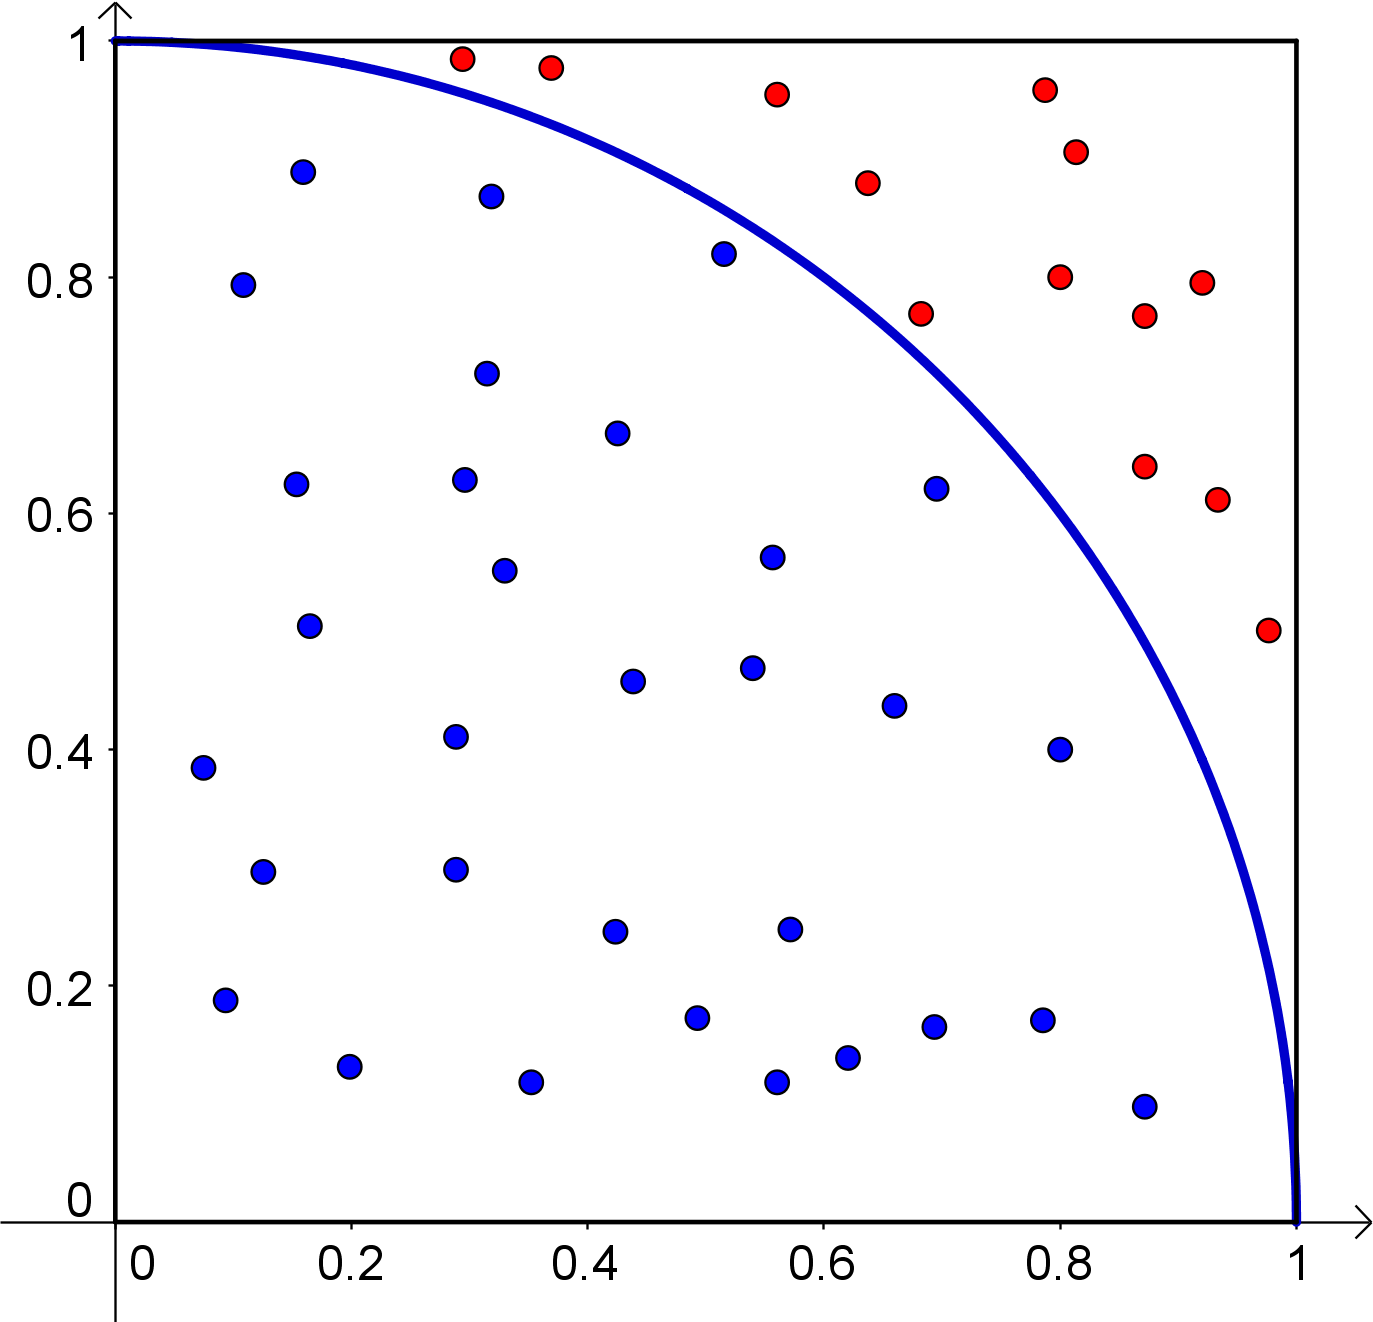
\includegraphics[width=0.4\textwidth]{fig/4_quartercircle_points.png}
	\caption{The area of the region is roughly the number of blue points divided by the total number of points generated. \label{fig:4_quartercircle_points}}
\end{figure}
\fi

This is easy to do.
Since the area under consideration is contained within the unit square $[0,1] \times [0,1]$, we can uniformly pick a point inside the square at random by using \texttt{RAND()} for each coordinate.
It is also simple to check whether a point is inside this circle: test if its distance from the origin is less than 1.
The following figures show the results of generating 20, 200, and 2000 points in this manner.

\begin{figure}[htbp]
    \begin{minipage}{0.3\textwidth}
        \centering
	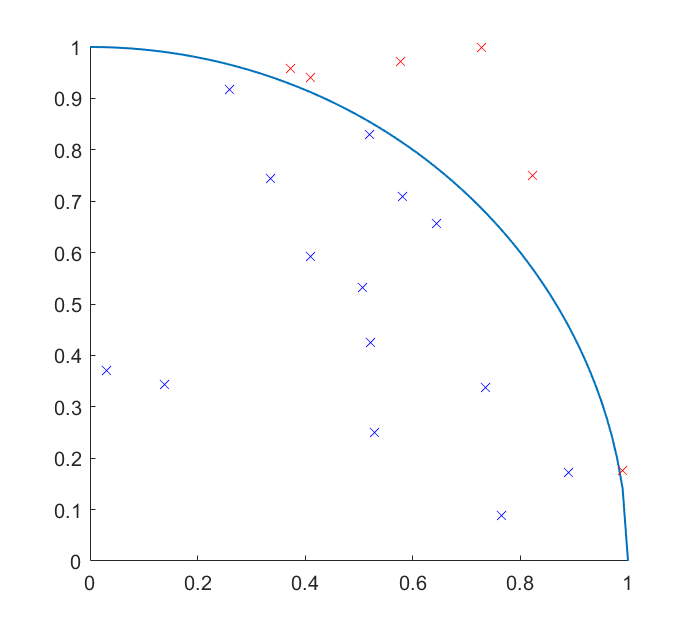
\includegraphics[width=\linewidth]{fig/4_quartercircle_1plot.png}
    \end{minipage}
    \hfill
    \begin{minipage}{0.3\textwidth}
        \centering
	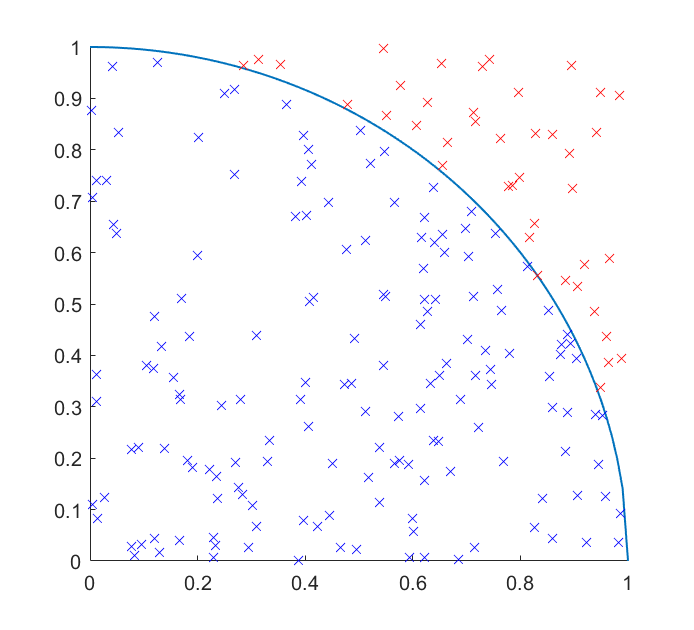
\includegraphics[width=\linewidth]{fig/4_quartercircle_2plot.png}
    \end{minipage}
    \hfill
    \begin{minipage}{0.3\textwidth}
        \centering
	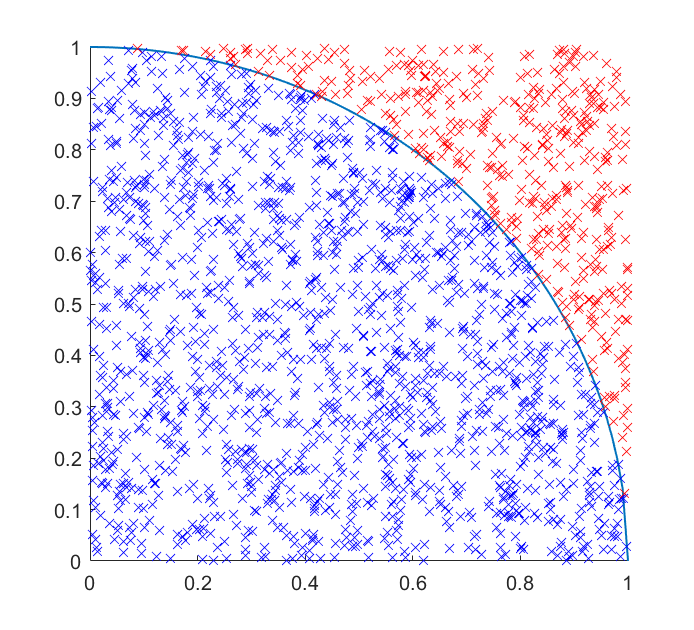
\includegraphics[width=\linewidth]{fig/4_quartercircle_3plot.png}
    \end{minipage}	
    \caption{20, 200, and 2000 randomly-generated points. \label{fig:4_quartercircleplots}}
\end{figure}

\newpage

\begin{figure}[htbp]
	\centering
	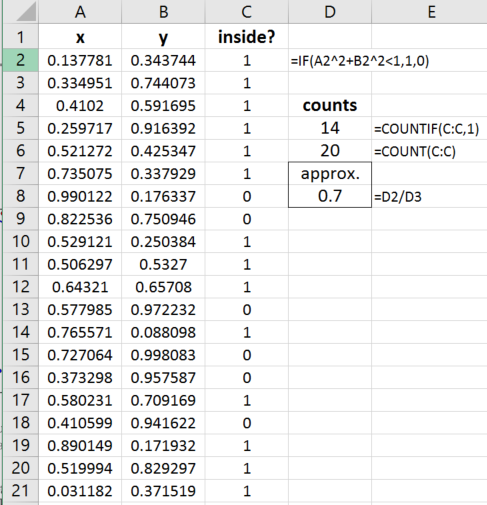
\includegraphics[width=0.5\textwidth]{fig/4_quartercircle_1.png}
	\caption{Area approximation of the quarter circle using 20 random points. \label{fig:4_quartercircle_1}}
\end{figure}

\begin{figure}[htbp]
    \begin{minipage}{0.45\textwidth}
        \centering
	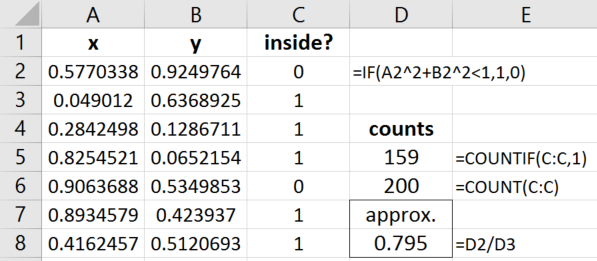
\includegraphics[width=\linewidth]{fig/4_quartercircle_2.png}
    \end{minipage}
    \hfill
    \begin{minipage}{0.45\textwidth}
        \centering
	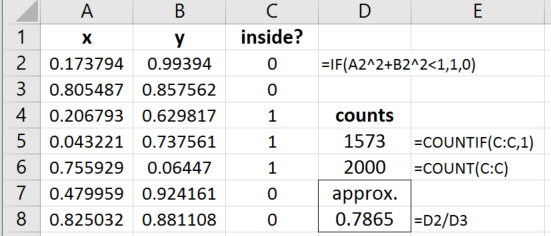
\includegraphics[width=\linewidth]{fig/4_quartercircle_3.png}
    \end{minipage}	
    \caption{Area approximations using 200 and 2000 random points. \label{fig:4_quartercircle_23}}
\end{figure}


A big advantage of this method is that it can be easily implemented when we have a way to test if a point in the set.
This is the case, for instance, if the set is the area under a curve.


Another approach to an area calculation like this involves breaking up the space $[0,1]\times[0,1]$ around the region into smaller squares, and colouring the squares whose centre is in the region under consideration -- see Figure~\ref{fig:4_heart} for an example.
Summing the areas of the coloured squares gives an estimate of the area; taking the limit of this as the squares get smaller is effectively equivalent to the integration technique from calculus.


\begin{figure}
\centering
    \begin{minipage}{0.3\textwidth}
        \centering
	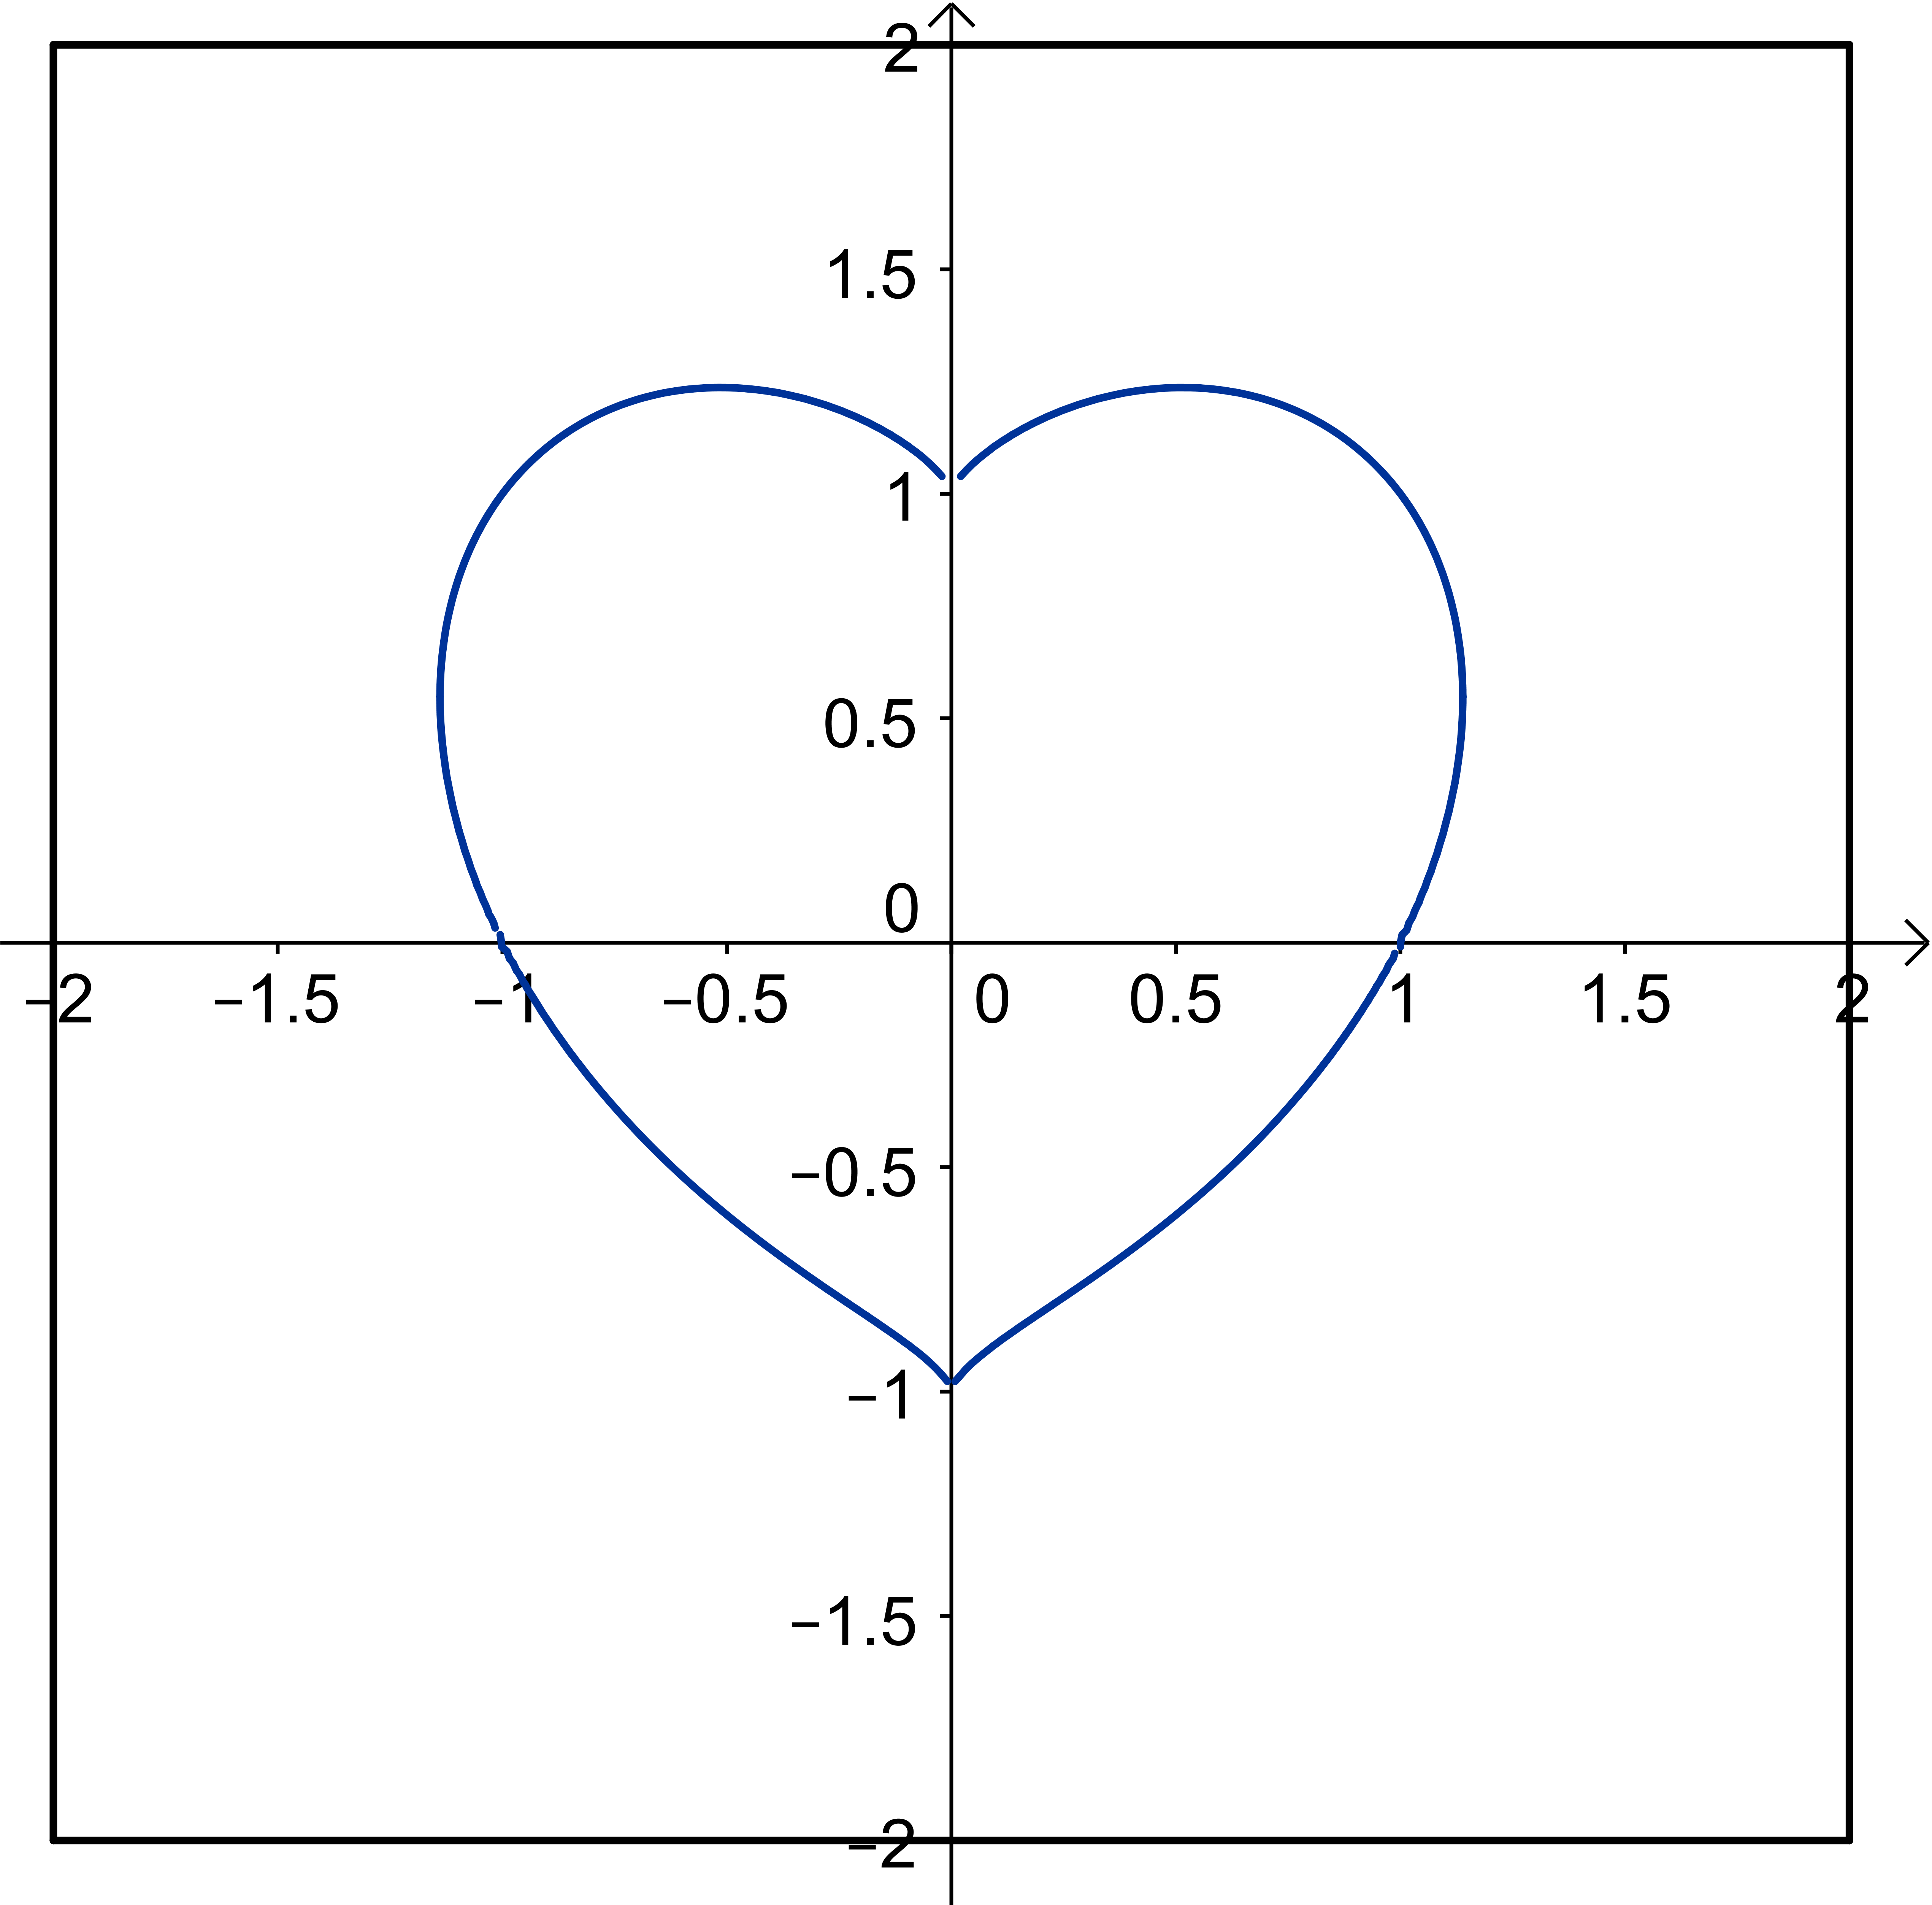
\includegraphics[width=0.85\linewidth]{fig/4_heart.png}
    \end{minipage}%
    \begin{minipage}{0.3\textwidth}
        \centering
	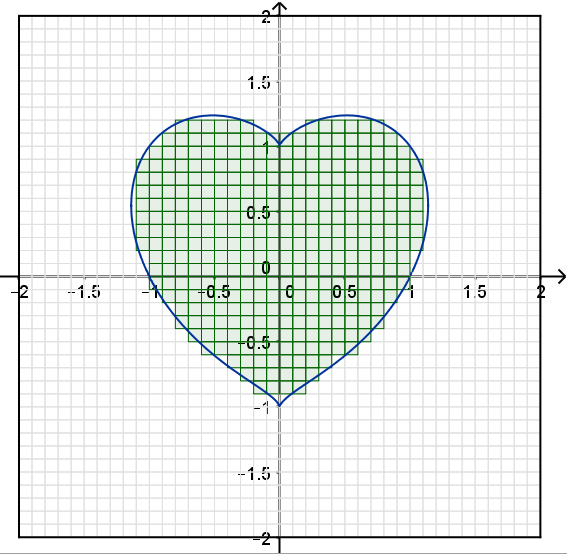
\includegraphics[width=0.85\linewidth]{fig/4_heart_sq.png}
    \end{minipage}	
    \caption{Approximating the area of a general region. \label{fig:4_heart}}
\end{figure}



But there are situations when one would prefer a random process (dropping points randomly and calculating the proportion) over a deterministic one (computing the integral, or estimating it from a count of grid points).
For instance, in two dimensions using an evenly-spaced grid makes sense, while in twenty-dimensional space it may not.
In particular, in high dimensions, grids have too many points: in dimension 20 the unit cube has over a million vertices and a $3 \times 3 \times \cdots \times 3$ grid has more than three trillion points while missing huge spaces inside the cube.
It is very difficult to find a deterministic way of producing well-spaced points in high dimension.
The method of using random points to estimate areas is called \emph{Monte Carlo integration}.


\section{The Normal Distribution, more PDFs and CDFs}\label{sec2:normal}

The \textbf{normal distribution} is often called the \textbf{Gaussian distribution} or the \textbf{bell curve}.
The two parameters associated with this distribution are the \emph{mean} $\mu$ and the \emph{standard deviation} $\sigma$.
Random variables drawn from this distribution will tend to be gathered around the mean, while the variance measures how `spread out' values are (a lower variance means values are more likely to stay close to the mean).
This distribution is denoted as $N(\mu, \sigma)$, and is one of the most important statistical distributions, because it is commonly seen in nature. For instance, in error analysis, measurement errors are modelled by the normal distribution (e.g. when calibrating instruments, etc).

In Figure~\ref{fig:2_normal} we show the probability density function of the standard normal distribution $N(0,1)$.
The density function for $N(\mu,\sigma)$ is 
$$f(x) = \frac{1}{\sigma\sqrt{2\pi}}e^{-\frac{1}{2}\left(\frac{x-\mu}{\sigma}\right)^2}.$$

\begin{figure}[htbp]
	\centering
	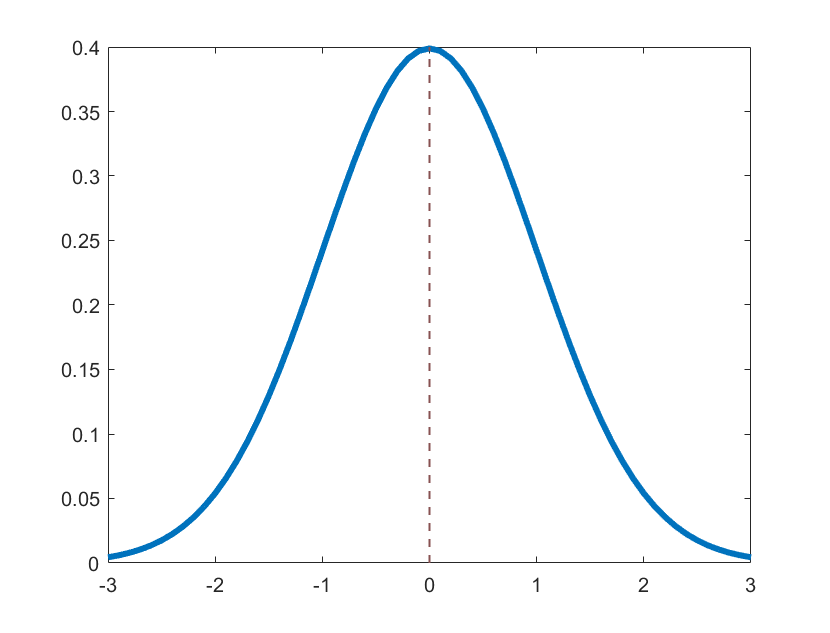
\includegraphics[width=0.5\textwidth]{fig/2_normal.png}
	\caption{The probability density function of the normal distribution $N(0,1)$ \label{fig:2_normal}}
\end{figure}

In Excel, the cumulative probability $P(Z < k)$ for $Z \sim N(\mu,\sigma)$ is calculated by the function \texttt{NORM.DIST(k,$\mu$,$\sigma$,cumulative)} function when the parameter \texttt{cumulative} is set to True (if it is set to False, it just outputs the value of the probability density function at that $k$). 
The function \texttt{NORMINV(prob,$\mu$,$\sigma$)} is the inverse of this; it calculates the point $k$ for which $P(Z < k) = $ \texttt{prob}.

\begin{figure}[htbp]
 \begin{minipage}{.5\textwidth}
        \centering
	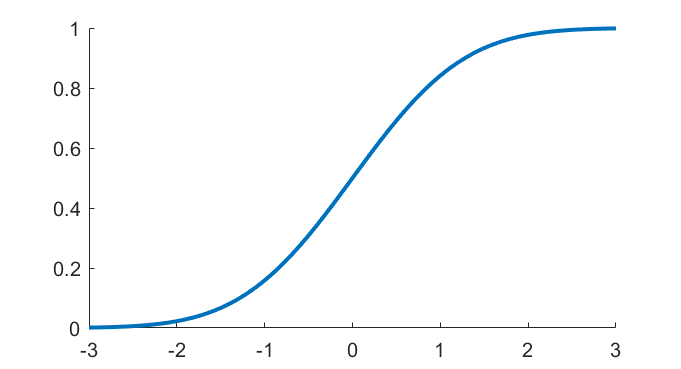
\includegraphics[width=0.9\linewidth]{fig/2_normal_cdf}
    \end{minipage}
    \begin{minipage}{0.5\textwidth}
        \centering
	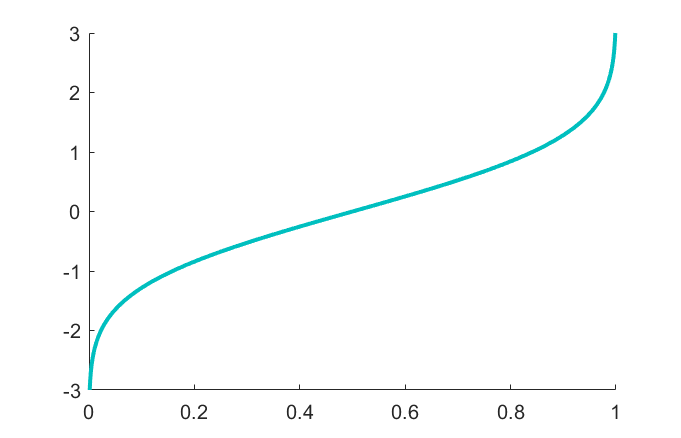
\includegraphics[width=0.9\linewidth]{fig/2_normal_cdf_inv}
    \end{minipage}	
    \caption{The cdf (L) and its inverse (R) for the standard normal distribution $N(0,1)$\label{fig:2_normal_cdf}}
\end{figure}

\begin{myexample}\label{ex:2_normal_example}
Suppose that we sample from a normal distribution with mean $\mu = 50$ and standard deviation $\sigma = 10$. What is the probability that the random sample is (a) smaller than 40? (b) in between 60 and 70?

\underline{Solution}
Using \texttt{NORM.DIST} in Excel, we can compute the required probabilities.
For (a), we get \texttt{NORM.DIST(40,50,10,TRUE)} $ = 0.158655$.
This is also equal to the area under the curve of $N(50,10)$ from $x = 0$ to $40$.

(b) This is calculated by the formula $$\texttt{NORM.DIST(70,50,10,TRUE)-NORM.DIST(60,50,10,TRUE)} = 0.135905,$$ and this is the area under the curve of $N(50,10)$ from $x = 60$ to $x = 70$. \qed
\end{myexample}

\begin{figure}[htbp]
 \begin{minipage}{.5\textwidth}
        \centering
	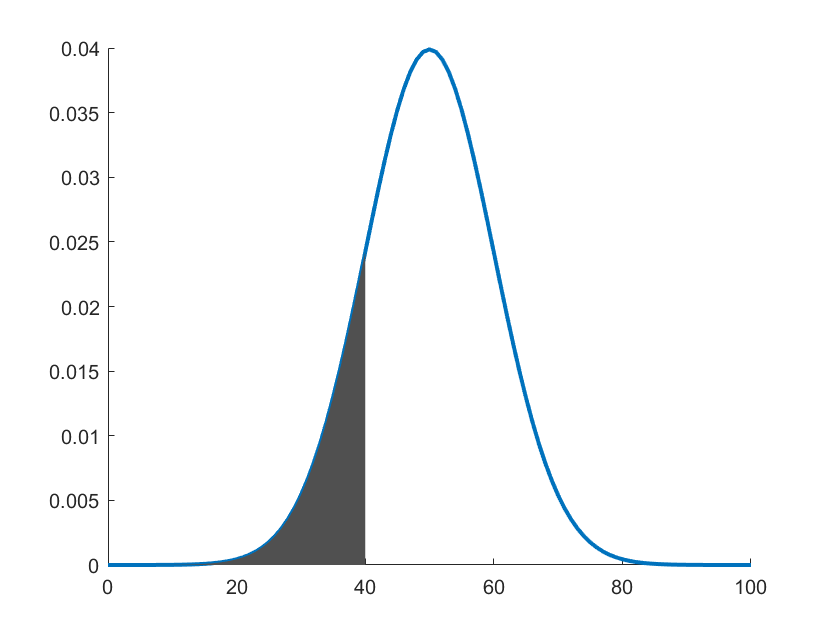
\includegraphics[width=0.9\linewidth]{fig/2_normal_example_a}
    \end{minipage}
    \begin{minipage}{0.5\textwidth}
        \centering
	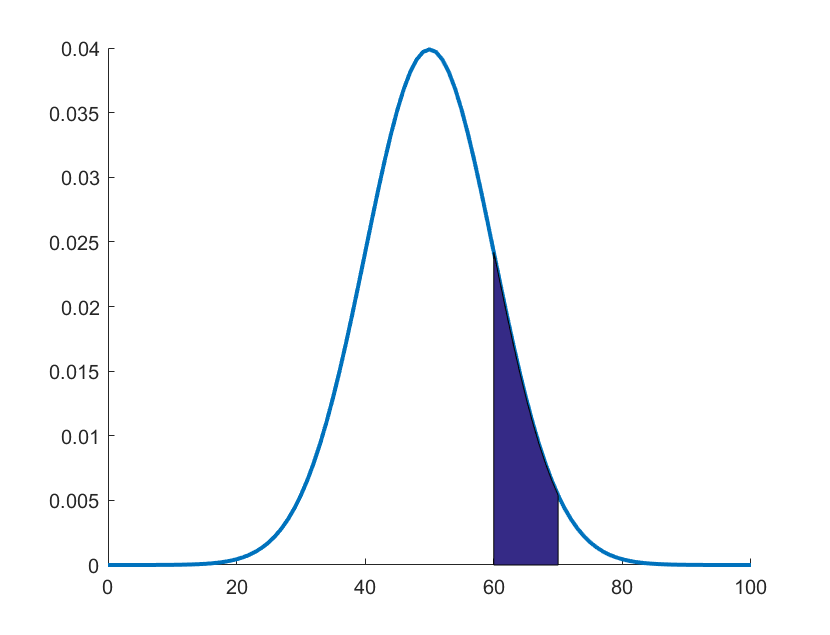
\includegraphics[width=0.9\linewidth]{fig/2_normal_example_b}
    \end{minipage}	
    \caption{The probabilities in Example~\ref{ex:2_normal_example} as areas under the normal curve \label{fig:2_normal_example}}
\end{figure}

To generate values from a normal distribution in Excel, one could just call the \texttt{NORMINV()} function with a random probability for its first argument.
For instance, the formula \texttt{NORMINV(RAND(),50,10)} will generate values from $N(50,10)$, as is illustrated in Figure~\ref{fig:2_normal_excel}.

\begin{figure}[htbp]
	\centering
	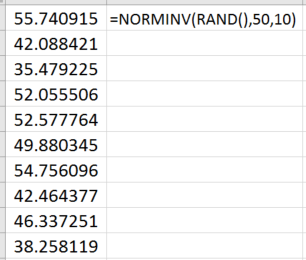
\includegraphics[width=0.3\textwidth]{fig/2_normal_excel.png}
	\caption{Generating values from $N(50,10)$ \label{fig:2_normal_excel}}
\end{figure}

\begin{myexample}
The heights of women in a certain country are normally-distributed with mean $\mu = 65$in and standard deviation $\sigma = 5$in. What is the probability that a randomly-selected person from this country is taller than 6ft?

\underline{Solution}: The probability is \texttt{1 - NORM.DIST(72,65,5,TRUE)} $ = .008076$, or 0.81\%. \qed
\end{myexample}

\section{The Exponential Distribution}\label{sec:2_expo}

The \textbf{exponential distribution} is another widely-used distribution in applications, since it models interarrival times between two events -- for example, the time it takes between customers at the bank, or the amount of time in between calls at a customer service centre.
It also models the lifetimes of electrical equipment.
This distribution is denoted as Exp$(\lambda)$, with the single parameter $\lambda > 0$ representing the average rate of arrivals/services per unit time.
The probability density function for Exp$(\lambda)$ is the following: 
\[f(x) = \left\{ \begin{matrix} \lambda e^{-\lambda x}, & x \geq 0 \cr 0, & \text{elsewhere} \end{matrix} \right. \]

\vspace{-0.5cm}

\begin{figure}[htbp]
	\centering
	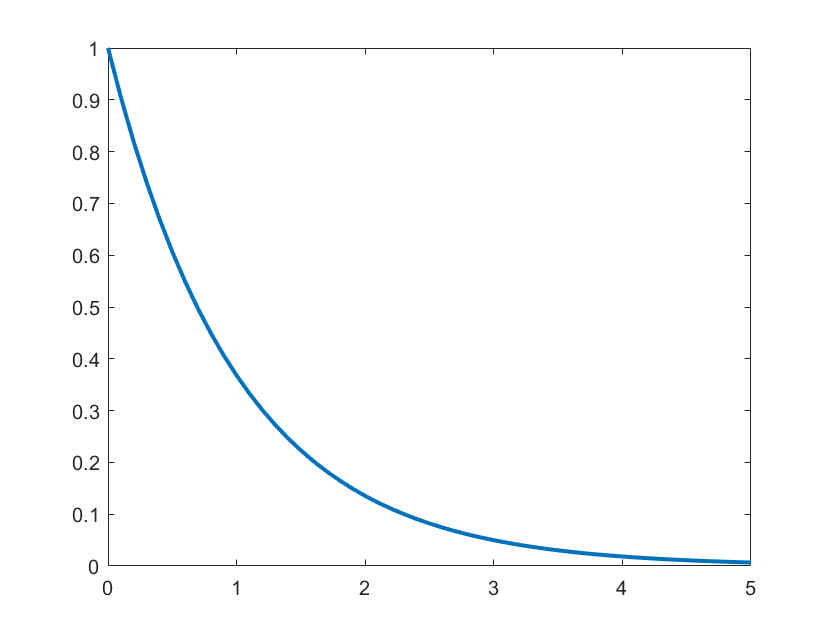
\includegraphics[width=0.5\textwidth]{fig/2_expo.png}
	\caption{The probability density function of the exponential distribution Exp$(1)$ \label{fig:2_expo}}
\end{figure}

As this is a continuous distribution, we will use cumulative probabilities $P(X < k)$ to describe events.
If $X \sim $ Exp$(\lambda)$, then its cdf is \[ P(X < k) = 1 - e^{-\lambda k}, k \geq 0.\]

\begin{myexample}\label{2:expo_example}
Suppose that 10 customers arrive at a restaurant per hour on average.
Find the probability that when the restaurant opens, the first customer arrives in the first 6 minutes.

\underline{Solution}: The interarrival times of customers is an exponentially-distributed random variable with $\lambda = 10$, or $X \sim \text{Exp}(10)$. Hence $P(X < 0.1) = 1 - e^{-10(0.1)} = 0.632121$, or 63.21\%. \qed
\end{myexample}

\begin{figure}[htbp]
	\centering
	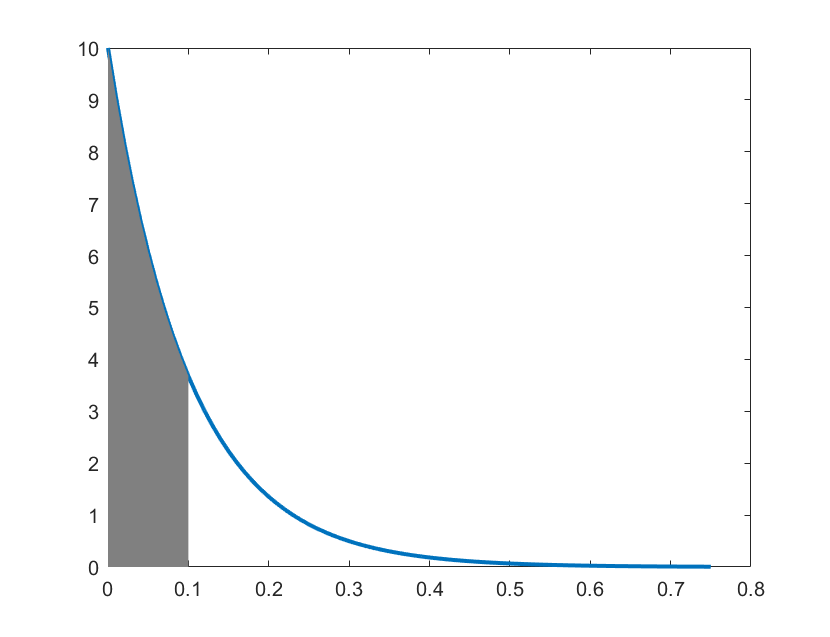
\includegraphics[width=0.5\textwidth]{fig/2_expo_example.png}
	\caption{The probability density function for Exp$(10)$ and the probability $P(X < 0.1)$. \label{fig:2_expo_example}}
\end{figure}


To calculate the cumulative probability $P(X < k)$ in Excel, the function is \\ \texttt{EXPON.DIST(k,lambda,TRUE)}, with the last parameter again indicating either the pdf (False) or the cdf (True).
However there is no built-in function for its inverse as in the normal distribution, since it has a simple algebraic expression: if $P(X < k) = y = 1 - e^{-\lambda k}$, then $k = -\frac{\ln(1-y)}{\lambda}$.
Hence we can randomly generate exponentially-distributed variables by using $y = $ \texttt{RAND()}, then computing $k$ from this expression.

\begin{figure}[htbp]
	\centering
	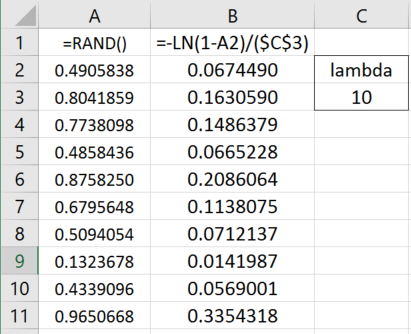
\includegraphics[width=0.4\textwidth]{fig/2_expo_excel.png}
	\caption{Ten values generated from Exp$(10)$ using \texttt{RAND()} and the inverse cumulative distribution function \label{fig:2_expo_excel}}
\end{figure}

One important property of the exponential function is that it is \emph{memoryless}, in that it models the time in between two events \emph{regardless of how many times that event has happened}.
In Example~\ref{2:expo_example}, this means that after the first customer has arrived, the time it takes for the second customer to arrive is also modelled by Exp($10$).
Similarly for the third, fourth, etc.
This is a common assumption when modelling queueing processes.

\iffalse

\section{The Poisson Distribution}

The \textbf{Poisson distribution} is a discrete distribution that is closely related to the exponential distribution.
For a Poisson-distributed random variable $X$ with parameter $\mu$, it has a \emph{probability density function} given by $$p(k) = P(X = k) = \left\{ \begin{matrix} \dfrac{e^{-\mu}\mu^k}{k!}, & k = 0,1,2,\ldots \cr \cr 0, & \text{ otherwise}\end{matrix} \right.$$
While the exponential distribution models waiting time in between two events, the Poisson distribution models the number of events that occur in a fixed time interval.
In fact, using this property we can use the exponential distribution to generate samples from the Poisson distribution:

Let $X \sim $ Pois$(\mu)$, and suppose $X_1, X_2, X_3, \ldots \sim $ Exp$(\mu)$.
Then $X = k$ if and only if \[ X_1 + X_2 + \cdots + X_k \leq 1 < X_1 + X_2 + \cdots + X_k + X_{k+1} \]

What this means is that to randomly generate from Pois$(\mu)$, we can generate values from Exp$(\mu)$ until their sum becomes larger than 1.
Then the Poisson value is one less than the number of values generated -- see Figure~\ref{fig:2_poisson}.

\begin{figure}[htbp]
	\centering
	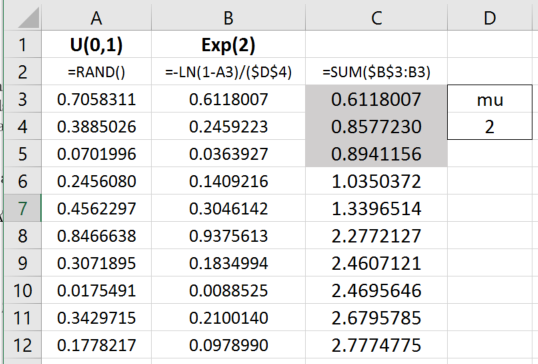
\includegraphics[width=0.5\textwidth]{fig/2_poisson.png}
	\caption{Generating a Poisson value randomly using the exponential distribution. Here the generated value is 3, since after 4 exponential values the sum becomes larger than 1. \label{fig:2_poisson}}
\end{figure}

This method is slightly more difficult to implement in Excel, especially for generating multiple Poisson values.
One would have to use some logical statements and checks (using the \texttt{IF()} function) to be able to do this multiple times.
In the next section we go over some features in Excel that allow us to generate multiple random variables.


\section{Data Tables}

To repeatedly generate random numbers in Excel, we use \textbf{data tables}.
These are used in Excel for scenario analysis -- recomputing a formula using different inputs.

\begin{myexample}
Suppose that for MATH208W your marks for each component are 30/40 for Assignments, 12/15 for the Midterm, and 20/20 for the Final Project.
Say you wanted to compute your final grade when your Final Exam mark is 5, 10, 15, 20, or 25/25.

First, input the individual components in Excel with a formula for the total, then create a column with the potential Final Exam marks you want to check.
In the column beside that, enter a formula referring to the output value you would like to track (\texttt{B5}).

\begin{figure}[htbp]
	\centering
	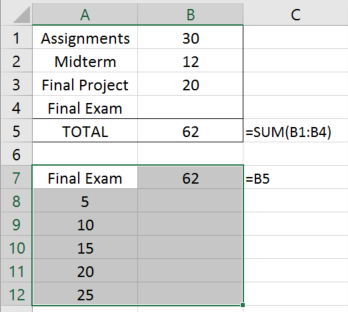
\includegraphics[width=0.5\textwidth]{fig/2_data_table_exA.png}
	\label{fig:2_data_table_exA}
\end{figure}

Next, highlight the two columns in the table you want to produce (in this example, \texttt{A7:B12}), then go to Data $\rightarrow$ What-If Analysis $\rightarrow$ Data Table.
For `column input cell' enter the cell whose value you would like to change.
Clicking Enter will generate the desired values.



\begin{figure}[htbp]
 \begin{minipage}{0.55\textwidth}
        \centering
	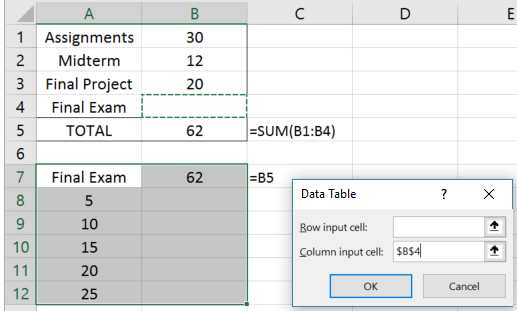
\includegraphics[width=\linewidth]{fig/2_data_table_exB.png}
    \end{minipage}
    \quad $\Rightarrow$ \quad
    \begin{minipage}{0.37\textwidth}
        \centering
	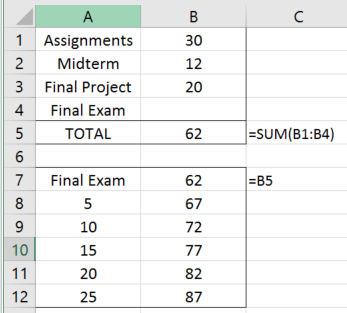
\includegraphics[width=\linewidth]{fig/2_data_table_exC.png}
    \end{minipage}	
    \caption{Using a data table in Excel. \label{fig:2_data_table_ex}}
\end{figure}

Note this is very basic; many real-world scenarios can be analyzed using this tool. \qed


\end{myexample}

Essentially, data tables do the work of entering information and recalculating the worksheet based on the changes.
For random number generation this is especially useful -- recall that each time the worksheet is refreshed/recomputed, each call to \texttt{RAND()} will refresh as well.

In Figure~\ref{fig:excel_binomial}, we generated a value from the binomial distribution $B(10,0.6)$.
By using a data table we can generate multiple values.
However since we are not changing any inputs (just refreshing the worksheet) the column input cell can be any empty cell.

\vspace{1cm}

\begin{figure}[htbp]
	\centering
	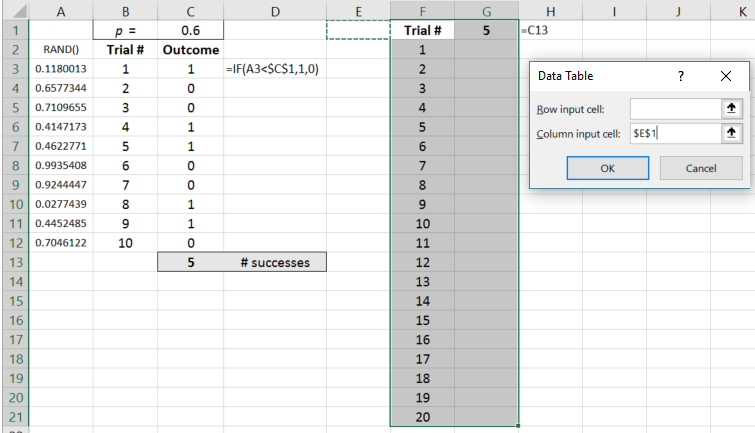
\includegraphics[width=0.9\textwidth]{fig/2_data_table_binomialA.png}
	\caption{Using a data table to generate binomial variates \label{fig:2_data_table_binomialA}}
\end{figure}

\begin{figure}[htbp]
	\centering
	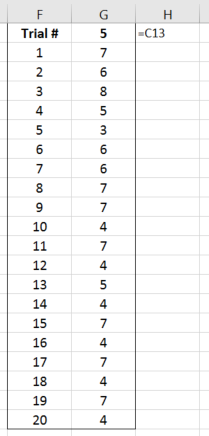
\includegraphics[width=0.3\textwidth]{fig/2_data_table_binomialB.png}
	\caption{Result of data table \label{fig:2_data_table_binomialB}}
\end{figure}

\fi

\newpage

\begin{center}
	\textbf{EXERCISES}
\end{center}

\begin{enumerate}[label={2.\arabic*},leftmargin=1cm]
	\item A pair of dice is rolled; let $X$ be the sum of the two numbers that appear. Tabulate the pdf for $X$. \label{2ex:pdf}
	\item Plot the cdf of the random variable $X$ of Exercise~\ref{2ex:pdf}
	\item \textbf{Explore}. We can simulate drawing a card at random from a standard deck of cards using $U\{1,52\}$, by assigning cards to numbers (1-13 are the A-K of clubs, 14-26 are diamonds, 27-39 hearts, and 40-52 spades).
		\begin{enumerate}[(a)]
			\item In Excel, generate 20 numbers from $U\{1,52\}$ and list the cards they correspond to. Do you see any repeats? How about when you generate 40 numbers?
			\item Guess the average number of draws from a deck of cards until \emph{the first repeat occurs}, assuming the draws are done with replacement. Run a few experiments to test your theory.
			\item Guess the average number of draws from a deck of cards until \emph{the first card is repeated}, assuming the draws are done with replacement. Again run some experiments on Excel to test your theory.
		\end{enumerate}
	      \item If $X \sim B(n,p)$, the probability that $X = k$ is known to be $$P(X = k) = \frac{n!}{k!(n-k)!}p^k(1-p)^{n-k}.$$ Use Excel to generate one hundred random variables from $B(20,0.7)$. Is your experiment consistent with this formula?
  \item A company that manufactures alarm clocks has determined that for each batch of 100 clocks produced, there are 5 that are defective. Suppose a clock is randomly selected from a batch of 100, and let $X$ be the random variable that is equal to 1 if this clock is defective, and 0 otherwise.
	  \begin{enumerate}
		  \item Determine the probability distribution of $X$ (with the associated parameter/s).
		  \item A clock is randomly selected from each of ten batches. What is the probability that none of the selected clocks are defective?
	  \end{enumerate}
  \item Suppose that the lifetime of a car's battery is exponentially distributed with parameter $\lambda = 1/1000$ hours. Use Excel to estimate the probability that (a) the battery fails before 500 hours of use; (b) the battery lasts longer than 750 hours but fails before 1200 hours.
  \item Two runners A and B run a race, and their running times are normally distributed with $N(60,8)$ and $N(65,5)$ (respectively).
	  \begin{enumerate}[(a)]
		  \item Use Excel to estimate the probability that runner A wins.
		  \item If runner C also joins the race, with running time distributed as $N(58,7)$, estimate the individual probabilities that each runner wins.
	  \end{enumerate}
  \item Using simulation, estimate the number of rolls needed in Exercise~\ref{2ex:pdf} until all possible values of $X$ (from 2 to 12) are seen.
	\item The heart-shaped region in Figure~\ref{fig:4_heart} is defined by the relation \vspace{-0.1cm}$$\{(x,y) : (x^2 + y^2 - 1)^3 - x^2y^3 \leq 0\}. \vspace{-0.1cm}$$
		Approximate its area using 1000 randomly-generated points in Excel.
	\item Choose three points uniformly at random on the unit circle $x^2 + y^2 = 1$.
		The probability that the triangle formed by these points contains the centre is $\frac{1}{4}$.
		Simulate this in Excel and verify this statement.

		Hint: To generate a point on a circle at random, generate an angle in $[0,2\pi)$.

		Hint \#2: You can fix one of the points to be at $(1,0)$
\end{enumerate}




\newpage

\chapter{Basic Simulations in Excel}\label{sec3}
\setlength{\epigraphwidth}{4in}
\epigraph{I am rarely happier than when spending an entire day programming my computer to perform automatically a task that would otherwise take me a good ten seconds to do by hand.}{Douglas Adams \& Mark Carwardine \\ \emph{Last Chance to See}, 1990}

Simulation is defined in \cite{banks2010} as \begin{quote} \emph{the imitation of the operation of a real-world process or system over time.} \end{quote}
There are many types of simulation, varying in the methods used and the type of systems being analyzed.
For instance, a simulation can be \emph{deterministic}, or \emph{stochastic}, depending on whether random variables are involved or not.
The first step in a simulation is usually to formulate the problem and the corresponding model -- here, assumptions will be made about the system being studied. 
This might include deciding which variables to ignore, or assuming how an input is distributed probabilistically.

In the previous sections, we discussed how to generate random variables in Excel, using a few of the most common probability distributions.
Before working on examples of simulations, we first discuss \textbf{data tables} in Excel.

\section{Data Tables in Excel}\label{sec3:datatable}

In Excel, data tables are used for scenario analysis.
They show the output of a calculation for different values of an input (similar to performing a sensitivity analysis).
We demonstrate this using an example.

\begin{myexample}\label{ex:3_datatable}
Suppose that you open a savings account at your bank on January 1 of this year, that earns you a fixed rate of 3\% per year.
If you deposit \$1,000 on January 1, at the end of the year you will have \$1,030.
What happens if we change the initial amount deposited?

Consider the following Excel spreadsheet: in cell \texttt{B2} we enter the initial amount deposited; \texttt{B3} has the interest earned (with formula \texttt{= 0.03 * B2}); \texttt{B4} has the total amount \texttt{= B2 + B3}.

To begin constructing the data table, in cells \texttt{D3:D14} input the different deposit amounts you would like to check (from \$900 to \$2,000).
In cell \texttt{E2} enter the formula \texttt{=B4}.

\begin{figure}[htbp]
	\centering
	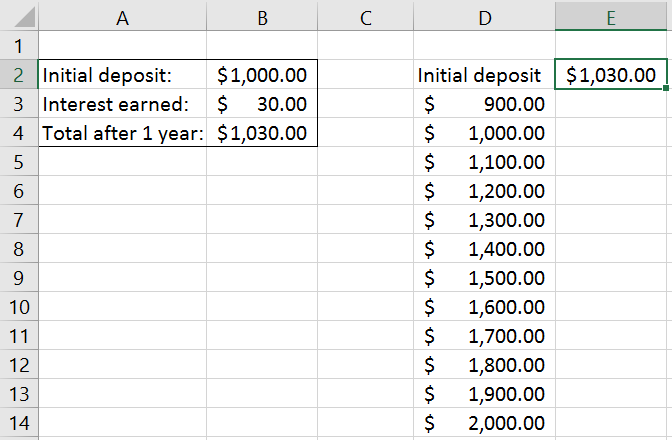
\includegraphics[width=0.45\textwidth]{fig/3_datatable_1.png}
	\label{fig:3_datatable_1}
\end{figure}

Now highlight cells \texttt{D2:E14}, and click `Data Table' (Data $\rightarrow$ What-If Analysis $\rightarrow$ Data Tables).
For `Column input cell' enter the cell corresponding to the initial deposit, \texttt{B2}, then click OK.

\begin{figure}[htbp]
	\centering
	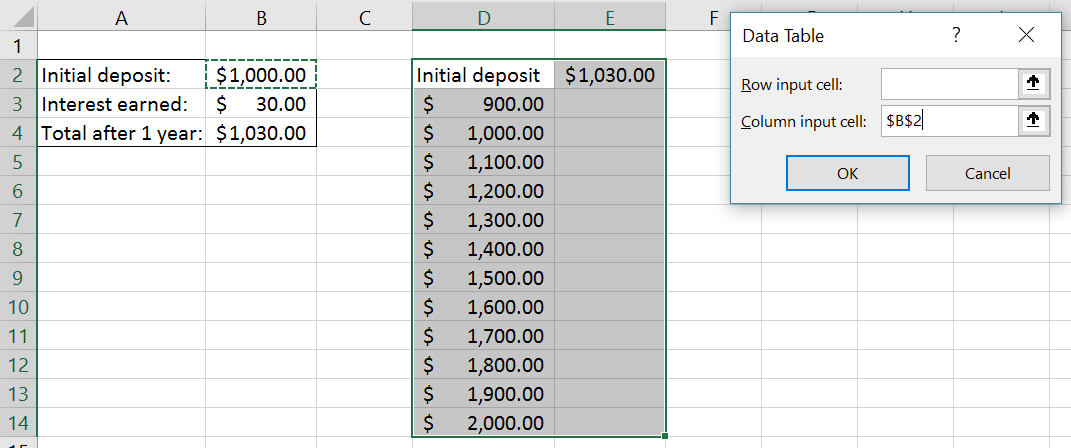
\includegraphics[width=0.75\textwidth]{fig/3_datatable_2.png}
	\label{fig:3_datatable_2}
\end{figure}

The cells beside the input column will be populated with the one-year totals for each corresponding initial deposit.

\begin{figure}[htbp]
	\centering
	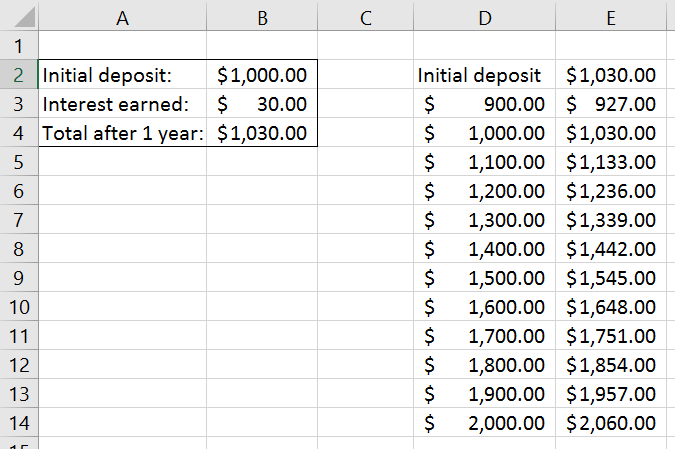
\includegraphics[width=0.5\textwidth]{fig/3_datatable_3.png}
	\label{fig:3_datatable_3}
\end{figure}

\end{myexample}

Data tables do the work of entering information and recalculating the worksheet based on the changes.
Example~\ref{ex:3_datatable} demonstrated a \emph{one-way data table}, because one input variable was allowed to vary.
We can also construct \emph{two-way data tables}.

\begin{myexample}\label{ex:3_datatable2}
Continuing the previous example, suppose that you wanted to compute your year-end savings account balance given different interest rates for the account.
To do this using a two-way data table, see the following spreadsheet:

\begin{figure}[htbp]
	\centering
	\includegraphics[width=0.9\textwidth]{fig/3_datatable2_1.png}
	\label{fig:3_datatable2_1}
\end{figure}

Enter the formula \texttt{=B4} in cell \texttt{D2}, and also change cell \texttt{B3} to the formula \texttt{=B1*B2}, to account for a varying interest rate.
In cells \texttt{E2:L2} enter the different interest rates under consideration.
Now highlight cells \texttt{D2:L14}, and click Data Table.
For `Column input cell' enter \texttt{B2}, and for `Row input cell' enter \texttt{B1}.

\begin{figure}[htbp]
	\centering
	\includegraphics[width=0.9\textwidth]{fig/3_datatable2_2.png}
	\label{fig:3_datatable2_2}
\end{figure}

Click OK.
The table should now be populated with the different year-end totals for the given combinations of initial deposit and interest rate.

\begin{figure}[htbp]
	\centering
	\includegraphics[width=0.9\textwidth]{fig/3_datatable2_3.png}
	\label{fig:3_datatable2_3}
\end{figure}


\end{myexample}

Rather than looking at an evenly-spaced set of input values, we can also construct tables based on random inputs to help us develop intuition for what the transformed random output should look like.

Note that Examples~\ref{ex:3_datatable} and ~\ref{ex:3_datatable2} are \emph{deterministic}: each entry has a value that is 
computed directly from its inputs, and repeating the calculation will produce an identical result.
The following example, on the other hand, is \emph{stochastic}: it incorporates some randomness.


\begin{myexample}\label{ex:3_datatable3}
Suppose that your initial deposit amount is a normally-distributed random variable with mean \$1,000 and standard deviation \$100.
In cell \texttt{B2}, following the discussion in Section~\ref{sec2:normal} we enter the formula \texttt{=NORM.INV(RAND(),1000,100)}.
To initialize the data table cell \texttt{E2} still refers to \texttt{B4}, while the first column can just have trial numbers (say we want to run this experiment 10 times).

\begin{figure}[htbp]
	\centering
	\includegraphics[width=0.4\textwidth]{fig/3_datatable3_1.png}
	\label{fig:3_datatable3_1}
\end{figure}

Highlight cells \texttt{D2:E12}, then click Data Table.
Now for `Column input cell' choose any blank cell.
The value in \texttt{B2}, and hence the output \texttt{B4}, will change each time the worksheet is recalculated so we do not need to specify a changing input cell.

\begin{figure}[htbp]
	\centering
	\includegraphics[width=0.7\textwidth]{fig/3_datatable3_2.png}
	\label{fig:3_datatable3_2}
\end{figure}

Click OK.
Now the table is populated by the different year-end values obtained given the assumption on the initial deposit.

\begin{figure}[htbp]
	\centering
	\includegraphics[width=0.5\textwidth]{fig/3_datatable3_3.png}
	\label{fig:3_datatable3_3}
\end{figure}
 

\end{myexample}

Now we begin our foray into simulation by looking at some simple problems.


\section{A Beginning Example -- Coin-Flipping}\label{sec3:begin}

The following problem recently appeared on the blog \emph{The Riddler}\footnote{A weekly puzzle blog on the site \texttt{http://www.fivethirtyeight.com}.}:

\begin{quote}
You and I find ourselves indoors one rainy afternoon, with nothing but some loose change in the couch cushions to entertain us. We decide that we'll take turns flipping a coin, and that the winner will be whoever flips 10 heads first. The winner gets to keep all the change in the couch! Predictably, an enormous argument erupts: We both want to be the one to go first.

What is the first flipper's advantage? In other words, what percentage of the time does the first flipper win this game?\footnote{\url{https://fivethirtyeight.com/features/can-you-time-the-stoplight-just-right/}, \\ January 20, 2017}
\end{quote}

This is a question about probability, and if you have taken some courses in probability and statistics, then you will  have seen exercises like this.
The exact probability that the first flipper wins the game can be computed analytically, but this is not easy to do.
However, the process is very simple to simulate.

To simulate the coin flips, we use a Bernoulli random variable with a $p = 0.50$ probability of heads.
Using 100 flips each, we keep track of the number of heads for each player, and compare the number of flips needed to get to 10.
Note that we have to cap the number of flips at a certain point, even though in theory there is a nonzero probability that neither player gets at least 10 heads in the first 100 flips.\footnote{Compute this probability using the inverse binomial function in Excel!}

\begin{figure}[htbp]
	\centering
	\includegraphics[width=0.7\textwidth]{fig/3_couch_1.png}
	\label{fig:3_couch_1}
\end{figure}

The formulas we use are: \texttt{RANDBETWEEN(0,1)} to generate the coin flips, and \texttt{SUM(\$B\$2:B2)} and \texttt{SUM(\$D\$2:D2)} for the running totals (autofilled).

To output the number of flips to get to 10, we use the \texttt{MATCH(lookup\_value, lookup\_array, [match\_type])} function in Excel, which finds the first occurrence of \texttt{lookup\_value} in the array \texttt{lookup\_array}, with parameter \texttt{match\_type} equal to 1, 0, or -1 depending on whether you want \texttt{MATCH} to find the first value less than or equal to, equal to, or greater than or equal to the lookup value, respectively.

In the spreadsheet shown, cell \texttt{H2} has the formula \texttt{MATCH(10,C2:C101,0)}, and cell \texttt{H3} has formula \texttt{MATCH(10,E2:E101,0)}.
In this run Player 1 gets 10 heads on the 17th flip, while Player 2 gets 10 heads on the 20th.
Lastly, in \texttt{H4} we enter the formula \texttt{IF(H2<=H3,1,2)}.


\begin{figure}[htbp]
	\centering
	\includegraphics[width=0.9\textwidth]{fig/3_couch_2.png}
	\label{fig:3_couch_2}
\end{figure}

To run this multiple times, we use a data table with 500 rows. 
We set a blank cell as the column input cell, as explained in Example~\ref{ex:3_datatable3}.

\begin{figure}[htbp]
	\centering
	\includegraphics[width=0.4\textwidth]{fig/3_couch_3.png}
	\label{fig:3_couch_3}
\end{figure}

Our results give 279 wins for Player 1, and 221 wins for Player 2.
Hence our simulation approximates the probability of Player 1 winning as $53.8\%$.
The actual probability is given by the expression \[ \sum_{n = 10}^\infty \left[\frac{1}{2^n}\frac{(n-1)!}{9!(n-10)!}  \left( 1 - \sum_{i=10}^{n-1} \frac{1}{2^i}\frac{(i-1)!}{9!(i-10)!}\right) \right] \approx 53.2909\%. \]
This is in some sense a ``lucky'' result, if you repeat the calculation you will see that it is usually not so accurate.

\section{Generating Permutations and Sampling without Replacement}

Here is another puzzle from \emph{The Riddler}:

\begin{quote}
On snowy afternoons, you like to play a solitaire `game' with a standard, randomly shuffled deck of 52 cards.
You start dealing cards face up, one at a time, into a pile.
As you deal each card, you also speak aloud, in order, the 13 card faces in a standard deck: ace, two, three, etc.
(When you get to king, you start over at ace.)
You keep doing this until the rank of the card you deal matches the rank you speak aloud, in which case you lose.
You win if you reach the end of the deck without any matches.

What is the probability you win?\footnote{\url{https://fivethirtyeight.com/features/can-you-deal-with-these-card-game-puzzles/}, \\ December 30, 2016.}
\end{quote}

One can compute solution exactly using combinatorics, but the calculation is difficult and subtle enough that the authors of the blog presented an oversimplified incorrect solution the following week, despite the fact that several people presumably sent the correct answer (while many others sent incorrect ones).\footnote{Original solution: \url{https://fivethirtyeight.com/features/dont-throw-out-that-calendar/}. \\ Correction: {\tiny \url{https://fivethirtyeight.com/features/how-long-will-it-take-to-blow-out-the-birthday-candles/\#correction}}. \\ Solution method: {\tiny \url{http://math.stackexchange.com/questions/1891958/derangements-of-a-deck-of-cards-where-ranks-are-equal}}, giving a probability of $1.6233\%$.}
Simulation can be a good sanity check on an analytic solution.
In this case, we would have to compute the solution quite accurately to spot the error.

To simulate this game, we need a way to generate a random arrangement of a 52-card deck.
Let us assign cards to numbers using the following scheme:

{ \small
\begin{center}	
\begin{tabular}{c|ccccccc}
& A & 2 & 3 & $\cdots$ & J & Q & K \\
\hline
$\spadesuit$ & 1 & 2 & 3 & $\cdots$ & 11 & 12 & 13 \\
$\vardiamond$ & 14 & 15 & 16 & $\cdots$ & 24 & 25 & 26 \\
$\varheart$ & 27 & 28 & 29 & $\cdots$ & 37 & 38 & 39 \\
$\clubsuit$ & 40 & 41 & 42 & $\cdots$ & 50 & 51 & 52 \\
\hline
(mod 13) & 1 & 2 & 3 & $\cdots$ & 11 & 12 & 0 
\end{tabular}
\end{center}
}

Note that we only have to consider these numbers modulo 13, since the suit is ignored.
Now we need to generate a random permutation of the numbers 1 to 52, corresponding to the shuffled deck of cards.

Refer to the spreadsheet below: first enter in cells \texttt{C2:C53} the numbers 1 to 52 -- this will correspond to the cards being announced.
Then, in the first column generate 52 random numbers using \texttt{RAND()}.
We then generate a permutation based on the relative positions of each cell in the array \texttt{A2:A53}.
To do this we enter in cell \texttt{B2} the formula \[\texttt{=INDEX(\$C\$2:\$C\$53,MATCH(LARGE(\$A\$2:\$A\$53,ROW()-ROW(\$A\$2)+1),\$A\$2:\$A\$53,0))}.\]
This instructs Excel to look for the $k$th largest entry in the array of random numbers, then output its relative position in that array.
Auto-filling the rest of the cells in \texttt{B2:B53} yields the random permutation.
In Figure~\ref{fig:3_deck_1}, for example, the first few cells in column B mean that the largest entry in column A is in the 6th position (\texttt{A7}), the second largest entry is in the 1st position (\texttt{A2}), and the third largest entry is in the 35th position.

\begin{figure}[htbp]
	\centering
	\includegraphics[width=0.25\textwidth]{fig/3_deck_1.png}
	\caption{Generating a random permutation in Excel. \label{fig:3_deck_1}}
\end{figure}

Observe that this method simulates sampling from a finite set without replacement, although generating a permutation is not practical for large sets.
Drawing only $k$ cards out of the deck without replacement corresponds to choosing the first $k$ entries in the permutation.

To check whether the drawn card matches the rank being called out, we just do a modulo check: \[ \texttt{=IF(MOD(B2,13)=MOD(C2,13),1,0)} \] will output 1 if the two ranks match, and 0 otherwise.
Summing up column C will result in the total number of times that the ranks match, so you win if this sum is zero.
Using a data table, we repeat this experiment 1000 times.


\begin{figure}[htbp]
	\centering
	\includegraphics[width=0.8\textwidth]{fig/3_deck_2.png}
	\label{fig:3_deck_2}
\end{figure}

The \texttt{COUNTIF} function in Excel counts how many instances of 0, 1, and so on, appear in the data table; as the spreadsheet shows we won 17 times out of 1000 trials (so we estimate the probability to be $1.7\%$).
More trials will lead to greater accuracy in estimating the true probability, which as noted is around $1.62\%$.

\section{Random Walks}

A \textbf{random walk} is a path where each step depends on a probability distribution.
Random walks have many applications, from physics (Brownian motion) to finance (movement of stocks on the market).

\subsection{Random Walks on a Line} 
A \emph{1-dimensional random walk} is a path on the real number line that starts at $0$, and with probability $p$ moves one unit to the right, and with probability $1-p$ moves one unit to the left.
Here we consider the simplest case, where $p = 0.5$.
We can think of each step as being determined by a fair coin flip.

\begin{figure}[htbp]
	\centering
	\includegraphics[width=0.5\textwidth]{fig/3_randomwalk_1.png}
	\label{fig:3_randomwalk_1}
\end{figure}

\vspace{-0.3cm}

This is easy to simulate in Excel, as shown in Figure~\ref{fig:3_randomwalk_2}.
Verify for yourself that the formula shown outputs \texttt{B1}$-1$ or \texttt{B1}$+1$ with equal probability.
Using the Chart function produces a visual of the random walk produced.

\begin{figure}[htbp]
	\centering
	\includegraphics[width=0.6\textwidth]{fig/3_randomwalk_2.png}
	\caption{Generating a random walk in Excel \label{fig:3_randomwalk_2}}
\end{figure}

A basic problem about random walks is whether they return to their starting point.
Let us generate random walks (using data tables) and then count what fraction of those generated do return to 0.
The next two figures show the results of generating a thousand random walks of length 100 and 1000, respectively.
Note the usage of the \texttt{MATCH} function to look for the first occurrence of zero in the walk.

\begin{figure}[htbp!]
	\centering
	\includegraphics[width=\textwidth]{fig/3_randomwalk_3.png}
	\caption{1000 random walks of length 100. \label{fig:3_randomwalk_3}}
\end{figure}


\begin{figure}[htbp!]
	\centering
	\includegraphics[width=\textwidth]{fig/3_randomwalk_4.png}
	\caption{1000 random walks of length 1000. \label{fig:3_randomwalk_4}}
\end{figure}

A \texttt{\#N/A} entry denotes that the walk did not return to 0, while the \texttt{COUNT} function counts the number of cells in the data table that have numbers.
Observe that only $92.2\%$ of the 100-step walks returned to 0, while $97.4\%$ of the 1000-step walks did.
This suggests that all the random walks will eventually return to zero, but some take a long time to do so.

We can also keep track of the average number of steps it takes for a walk to return to zero.
We calculate this using \texttt{AVERAGEIF(G2:G1001,``>=0'')}, which takes the average of the cells in the data table while ignoring the cells with \texttt{\#N/A}.
Increasing the length of the walk thus increases the number of walks that do return to zero, but the average number of steps continues to increase as we increase the number of steps and capture the walks that take a long time to return to zero.
In fact, it is possible to prove (with considerable effort) that while walks will eventually return to zero, the expected time to return is infinite.
This is because the average time is dominated by a few long walks, a fact that we can appreciate experimentally.

\newpage

Using Python we generated 100,000 walks for each of the following lengths, and obtained these results. (The code to implement this can be found after the exercises.)

\begin{center}
\begin{tabular}{rcr}
length of walks & \% returning & average time to return\\
\hline
10 & $73.513\%$ & $3.27$ \\
100 & $92.049\%$ & $8.57$ \\
1000 & $97.471\%$ & $25.86$ \\
10000 & $99.183\%$ & $76.30$ \\
100000 & $99.744\%$ & $238.20$ \\
1000000 & $99.932\%$ & $786.75$ \\
10000000 & $99.976\%$ & $2949.73$ \\
\end{tabular}
\end{center}

Observe that even for walks with ten million steps there is a small fraction that do not return to zero.

Using the same simulation we can also investigate the expected distance from the origin after a fixed number of steps.
Try this yourself for walks of 100 steps and then 1000 steps, and try to understand the pattern.



\subsection{Random Walks on a Grid}

Suppose now that we start at the origin $(0,0)$ in 2-dimensional space, and consider the lattice of integer points $\{(x,y) : x,y \text{ integers}\}$.
Assume that there is an equal probability (of $0.25$ each) of moving to an adjacent integer point at each step.
We would now like to estimate similar quantities as in the 1-dimensional case: what is the probability of returning to the origin?
What is the expected distance from the origin for a walk of fixed length?
We remark that the expected time to return to zero must be $\infty$ as it is that for each coordinate separately.
Moreover there are multiple notions of distance we can consider -- the Euclidean distance ($\sqrt{x^2 + y^2}$) and the Manhattan distance ($|x| + |y|$) are examples.

\begin{figure}[h]
	\centering
	\includegraphics[width=0.5\textwidth]{fig/3_random2D_2.png}
	\caption{100 steps of a random walk on a grid, visualized. \label{fig:3_random2D_2}}
\end{figure}


To simulate this in Excel, we now need to keep track of two columns, one each for the $x$- and $y$-coordinate.
Refer to Figure~\ref{fig:3_random2D_1} for the formulas used (note that \texttt{F2} has a formula that changes based on the length of this walk, which is input in \texttt{F5}).

\vspace{0.5cm}

\begin{figure}[h]
	\centering
	\includegraphics[width=\textwidth]{fig/3_random2D_1.png}
	\caption{100 steps of a random walk on a grid. \label{fig:3_random2D_1}}
\end{figure}

\vspace{0.5cm}

Using a data table, we simulate a thousand random walks of length 100 and 1000.
Observe that the percentages are much smaller than what we saw in the one-dimensional case: $58.1\%$ for walks of length 100, and $69.9\%$ for walks of length 1000.
Even increasing the length to 5000 only increases this observed frequency to $71.8\%$ (try it yourself and see what percentages you get!).

\vspace{0.5cm}

\begin{figure}[h]
	\centering
	\includegraphics[width=\textwidth]{fig/3_random2D_3.png}
	\caption{1000 random walks of length 100. \label{fig:3_random2D_3}}
\end{figure}

\vspace{0.5cm}

\begin{figure}[h]
	\centering
	\includegraphics[width=\textwidth]{fig/3_random2D_4.png}
	\caption{1000 random walks of length 1000. \label{fig:3_random2D_4}}
\end{figure}

Based on this, it is hard to tell if the probability of returning to the origin might be smaller than 1 -- however, it has been shown analytically that as the length of the walk approaches infinity, this probability approaches 1.\footnote{See the article on \emph{P\'olya's Random Walk Constants} at \\ \url{http://mathworld.wolfram.com/PolyasRandomWalkConstants.html}.}
This illustrates one difficulty of performing simulations -- if the sample size is too small, the results might not necessarily reflect the true behaviour accurately.
In this example, even working with walks of length 5000, we still found a return rate of smaller than $75\%$.
On the other hand, it is hard to run a large number of experiments on Excel, as we don't have a good way to truncate walks that have already returned to zero.
Other programming languages are better for this purpose, however the trade-off between accuracy and running time remains.

\vspace{1cm}

\begin{center}
	\textbf{EXERCISES}
\end{center}

\begin{enumerate}[label={3.\arabic*},leftmargin=1cm]
	\item Consider the following experiment: roll three 6-sided dice at the same time, and let $X$ be the random variable that is equal to the number of different outcomes seen. For example, a roll of $\{3, 5, 5\}$ gives $X = 2$. Estimate the probability distribution for $X$ using an Excel simulation. Then, by enumerating all possibilities completely, determine the exact probabilities.
	\item Another puzzle from \emph{The Riddler}:
		\begin{quote}
			You and I stumble across a 100-sided die in our local game shop.
		We know we need to have this die -- there is no question about it -- but we're not quite sure what to do with it.
		So we devise a simple game: We keep rolling our new purchase until one roll shows a number smaller than the one before.
		Suppose I give you a dollar every time you roll.
		How much money do you expect to win?\footnote{\url{https://fivethirtyeight.com/features/how-long-will-it-take-to-blow-out-the-birthday-candles/}, January 13, 2017.}
	\end{quote}
		Estimate this quantity using a simulation.
	      \item The probability that two positive integers picked randomly are coprime (that is, they share no divisors other than 1) is $\frac{6}{\pi^2}$.
		Provide estimates for $\pi$ by taking 100, 1000, and 10000 pairs of integers from the ranges $\{1,2,\ldots,100\}$, $\{1,2,\ldots,1000\}$, and $\{1,2,\ldots,10000\}$.\footnote{This video by mathematician-comedian Matt Parker on his \emph{Youtube} channel \emph{standupmaths} demonstrates this process: \url{https://www.youtube.com/watch?v=RZBhSi\_PwHU} .}
	\item For a random walk in one dimension, estimate the expected distance from the origin after 200, 500, and 1000 steps by generating 1000 walks for each case.
	\item \textbf{Biased random walks}. Consider a one-dimensional random walk where you move one unit to the left with probability $p$ and one unit to the right with probability $1 - p$.
		Simulate this for $p = 0.6$.
		Do you expect all walks to return to the origin in this case?
		How about if $p = 0.8$?
	\item \textbf{Biased random walks}. Consider a one-dimensional random walk where at the origin, you move one unit to the left or right with equal probability, but everywhere else, you move \emph{towards the origin} with probability $p$, and \emph{away from the origin} with probability $1-p$.
		Simulate this for $p = 0.4$ and $p = 0.6$, and explain your results.
		Note that the formula to generate the next step is more involved, since you have to deal with three different cases.
	\item \textbf{Random walks in three dimensions}.
		Consider a random walk in 3D, where you start at the origin $(0,0,0)$, and with equal probability move $1$ or $-1$ units in one of the coordinate directions.
		Simulate this in Excel for a maximum length of 100 steps, and generate 100 walks using a data table. How many return to the origin?
		Try to generate longer walks (as far as your computer allows).
		Can you make any conclusions?

\end{enumerate}


{\small

\textbf{Python code for generating random walks}
\vspace{-0.5cm}

\begin{verbatim}
from __future__ import division
import random as rd

def randwalk(N,p=0.5,marker=0):
# Function for generating a random walk
# Input: N, p (prob of -1 step), marker (starting point)
#      *defaults are p = 0.5 and marker = 0
# Output: number of steps to first return to origin 
#         (or 0 if it does not return)
    current = marker # Initialize
    count = 0
    while count < N:
        # Generate random numbers, and move left or right
	# corresponding to probabilities
        r = rd.random()
        if r < p:
            current -= 1
        else:
            current += 1
        count += 1
        if current == 0:
            return count
    return 0


# Now aggregate up to M walks, and take return rate in % 
# and the average # steps to return

# Initialize parameters
N = 100
p = 0.5 
marker = 0
M = 100000 # Number of walks to aggregate

total_returns = 0
total_steps = 0
counter = 0

while counter < M:
    steps = randwalk(N,p,marker)
    if steps > 0:
        total_returns += 1
        total_steps += steps
    counter += 1

average_steps = total_steps/total_returns
return_rate = 100*total_returns/M

print "%d random walks of length %d were generated." % (M, N)
print "%7.4f%% of all walks returned to 0." % (return_rate)
print "On average it took %10.2f steps to return." % (average_steps)
\end{verbatim}

}






\newpage

\chapter{An Introduction to Queueing Theory}\label{se:queueing}
\setlength{\epigraphwidth}{4.25in}
\epigraph{3.~There is no point in waiting at the end of the line. \\ 4.~If you don't wait at the end of the line, you'll never get to the front. }{Charles Wright\\ \emph{Wright's Axioms of Queueing Theory}}



\section{A Framework for Simulation}

The goal of simulation is the analysis of a real-world process by imitating its behaviour using computer software.
In the previous chapters we saw examples of how we could use randomness to perform calculations that are deterministic in nature (e.g. the area calculations in Section~\ref{sec2:areavolume}).
Such experiments are referred to as \textbf{Monte Carlo Methods}.

Moreover, we also performed simulations of processes for which randomness was an inherent characteristic (rolling a die, etc., in Chapter~\ref{sec3}).
Arguably this scenario is more interesting than the former, since one cannot \emph{solve} these processes analytically as one can theoretically do for area and volume calculations; outcomes of these experiments cannot be predicted (although one can derive quantities like the long-term behaviour of random processes).
And herein lies the main advantage of simulation -- it is a low-risk method for obtaining knowledge about how a random system operates (or \emph{will operate}).

In particular, \underline{what if} questions are addressed easily by simulations.
\emph{What if we change one of the starting assumptions?}
\emph{What if we remove a certain part of the system?}
These are not easy to analyze in general, but simulations may reveal what the outcomes are.

In \cite{banks2010} some commonly-used terms in simulations are defined:

\begin{itemize}
	\item \emph{system}: A group of objects that interact with each other or are interdependent, joined together to work toward a common goal.
	\item \emph{system environment}: Where the system is `located,' i.e. refers to the space outside the system but from where changes to the system can be caused.
	\item \emph{entity}: An object in the system.
	\item \emph{attribute}: A property of an entity.
	\item \emph{activity}: A time period of given length.
	\item \emph{state}: The collection of variables necessary to describe the system at any given time.
	\item \emph{event}: An instantaneous occurrence that might change the state of the system.
	\item \emph{model}: A representation of the system.
\end{itemize}

There are a few more classifications that are used to refer to systems and their simulation.

\begin{itemize}
	\item A system is \emph{discrete} if changes can only happen at a discrete set of time points, and \emph{continuous} if variables can change continuously.
	\item A simulation model is \emph{static} if it represents a system at a fixed point in time, and \emph{dynamic} if it represents a system as it changes over time.
	\item A model is called \emph{stochastic} if it contains random variables, and \emph{deterministic} otherwise.
\end{itemize}

Note that we can also refer to models as discrete or continuous, and that the type of model used may not necessarily match the type of system being observed (so a discrete model can be used to study a continuous system, and vice versa).
The term \textbf{discrete-event simulation} refers to the case when the types of models studied are discrete, dynamic, and stochastic.

Typically, simulation-based studies will follow the same framework.
First, a problem is identified and formulated.
Then, objectives are set -- what do we want to know?
Is simulation the appropriate tool?
Then a model is formulated; this may be a very involved process, and there is no single approach that will work for all problems.
In general, it is a good idea to start with a simple model, and then increase the complexity as the study moves forward.

Once the model is constructed, input data is collected, and the model programmed into a computer.
Then \emph{model verification} and \emph{model validation} are done.
This means that the model is first checked, to make sure the data representations used are appropriate, and the logic is sound (verification).
Then, the model is run on a few test cases where the real-world outcome is known, and the outputs are compared (validation).

After these steps, the actual experiment begins.
Parameters such as the maximum number of iterations, maximum time of simulation, and number of replications of each run are fixed, and input data is selected.
Then the model is run, and an analysis is carried-out on the system being studied.


\newpage

\section{Simulating Simple Queues}

Queueing is something everyone experiences in daily life -- we wait in lines at the supermarket, at the bank, when taking transit, and so on.
Routers also queue information to send to your wireless devices.
Modelling the behaviour of queues can be very involved and complicated, especially for more complex systems.
When studying a system with queues, we are interested in various properties of such as:

\begin{enumerate}[(1)]
	\item Average waiting times,
	\item Average total times in the system (including the processing time),
	\item Average size of queues,
	\item Probability of spending time in a given queue,
	\item Proportion of idle time of the server.
\end{enumerate}


To understand a queueing system, we should model arrival times for \emph{customers}, their routes through the system, and \emph{service times} once a customer is being processed.
For instance, at a supermarket we might want to analyze its queueing system for checking out.
This would involve gathering data empirically to determine what probability distribution governs the time between two customer arrivals at the queue (which may vary depending on time of day) and studying how long it takes to serve a customer.
This analysis could then be used to predict the effects of adding counters or varying the checkout procedures, e.g. through introducing express counters or self-checkout counters.

The following assumptions are typical in simple queueing models:
\begin{enumerate}[(a)]
	\item Interarrival times of the customers are drawn independently from some probability distribution $A$.
	\item Service times of successive customers are drawn independently from some probability distribution $S$.
	\item When a customer arrives and the server is idle, the customer is immediately served.
		Otherwise, if the server is busy, the customer joins the end of the queue.
\end{enumerate}

Key characteristics that differentiate one queueing system from another are the probability distributions for arrivals and service time, and the number of servers.
For now we limit our discussion to single-server queues.

\vspace{0.5cm}
\begin{figure}[htbp]
	\centering
	\includegraphics[width=0.9\textwidth]{fig/4_queuepaint0.png}
	\caption{A single-server queue. \label{fig:4_queuepaint0}}
\end{figure}

\vspace{0.4cm}

\newpage

\begin{myexample}\label{ex:4_queue}
	In a single-server queue, interarrival times follow the discrete uniform distribution $U\{1,6\}$.
	Customers are served in 3 minutes with probability $0.25$, 4 minutes with probability $0.5$, and 7 minutes with probability $0.25$.
	Simulate this process until 10 customers are served, and find the average waiting time of a customer.

First, we have to generate interarrival times. 
Suppose that we used Excel to do this, and obtained the following: 4, 3, 5, 5, 5, 1, 4, 2, 5, 3 (using the \texttt{=RANDBETWEEN()} function).

Next, we generate service times, and obtain: 4, 7, 4, 3, 3, 3, 4, 7, 4, 4 (using the \texttt{IF()} function with \texttt{RAND()}).

Assuming we start at time $t = 0$, the first customer arrives at time $t = 4$.
Since the server is idle when he arrives, he is served immediately. 


\begin{figure}[htbp]
	\centering
	\includegraphics[width=0.8\textwidth]{fig/4_queue_ex1a.png}
	\caption{State of the system at $t = 4$. \label{fig:4_queue_ex1a}}
\end{figure}

The service time for the first customer is 4 minutes.
Before he finishes being served, however, the second customer arrives at time $t = 4 + 3 = 7$.


\begin{figure}[htbp]
	\centering
	\includegraphics[width=0.8\textwidth]{fig/4_queue_ex1b.png}
	\caption{State of the system at $t = 7$. \label{fig:4_queue_ex1b}}
\end{figure}


The first customer exits the system at $t = 8$, at which point the second customer is served, with service time $7$ minutes.
The third customer arrives at time $t = 12$, and has to wait in the queue for 3 minutes until the second customer exits.

\begin{figure}[htbp]
	\centering
	\includegraphics[width=0.8\textwidth]{fig/4_queue_ex1c.png}
	\caption{States of the system at $t = 8$ and $t = 12$. \label{fig:4_queue_ex1c}}
\end{figure}

The rest of the system behaviour can be derived similarly.
Putting everything in a table, we obtain the following values.
The waiting time of a customer is the time between arrival time and when service begins, while the total time in the system is the sum of the waiting time and the service time.

{\small
\begin{center}
\begin{tabular}{cccccccc}
	\multirow{2}{*}{Customer} & Interarrival & Time of & Service & Service & Service & Waiting & Total time \\
	& times & arrival & time & start & end & time & in system \\
\hline
1 & 4 & 4 & 4 & 4 & 8 & 0 & 4 \\
2 & 3 & 7 & 7 & 8 & 15 & 1 & 8 \\
3 & 5 & 12 & 4 & 15 & 19 & 3 & 7 \\
4 & 5 & 17 & 3 & 19 & 22 & 2 & 5 \\
5 & 5 & 22 & 3 & 22 & 25 & 0 & 3 \\
6 & 1 & 23 & 3 & 25 & 28 & 2 & 5 \\
7 & 4 & 27 & 4 & 28 & 32 & 1 & 5 \\
8 & 2 & 29 & 7 & 32 & 39 & 3 & 10 \\
9 & 5 & 34 & 4 & 39 & 43 & 5 & 9 \\
10 & 3 & 37 & 4 & 43 & 47 & 6 & 10
\end{tabular}
\end{center}
}

The average waiting time of a customer in this system is therefore 2.3 minutes, while the average time a customer spends in the system is 6.6 minutes.
Certainly, the table can (and should) be calculated using Excel.
The long-run averages can be computed analytically -- however in this example, in the long run the queue will grow as the average service time is longer than the average interarrival time, meaning the long-run wait times diverge to infinity.
However this behaviour may not be apparent when simulating only a limited number of customers in Excel. \qed


\end{myexample}

In general, queues are represented using the notation A/S/$n$, where A represents the arrival time distribution, S the service time distribution, and $n$ the number of servers.

When interarrival times and service times are both exponentially distributed, we call the queue an M/M/$n$ queue (where `M' stands for \emph{memoryless} or \emph{Markov}).
This is one of the simplest types of queue to analyze, and provides a convenient model for many applications.
Conventionally, the parameters for these distributions are called $\lambda$ and $\mu$ (so interarrival times are Exp($\lambda$) and service times are Exp($\mu$)).


The queue in Example~\ref{ex:4_queue} can be referred to as a G/G/1 queue, where G stands for general probability distribution -- that is, it is not one of the common ones encountered.
\footnote{See the wiki page \url{https://en.wikipedia.org/wiki/Kendall's\_notation}.}

\iffalse
\begin{figure}[htbp]
	\centering
	\includegraphics[width=0.8\textwidth]{fig/4_queuepaint.png}
	\caption{An M/M/1 queue. \label{fig:4_queuepaint}}
\end{figure}
\fi

\begin{figure}[htbp]
	\centering
	\includegraphics[width=0.6\textwidth]{fig/4_queuepaintMMn.png}
	\caption{An M/M/$n$ queue. \label{fig:4_queuepaintMMn}}
\end{figure}


\begin{myexample}\label{ex:4_MM1}
	Suppose that a queue follows the M/M/1 model with interarrival times distributed as Exp($3$) and service times distributed as Exp($5$), where a unit of time is 1 hour.
	This means that on average, 3 customers arrive in an hour, and the server can serve 5 customers in an hour,
 i.e.~$\lambda=3$ and $\mu=5$.
	Simulate this queue for 20 customers and compute the average waiting time and the average total time in the system for a customer.


To simulate this in Excel, we need to generate two sequences of values from Exp($\lambda$) and Exp($\mu$), and use these values to calculate waiting times and other statistics about the system.
Recall that we use the formula $-\frac{\ln(1-\texttt{RAND()})}{\lambda}$ to sample from Exp($\lambda$).
The spreadsheet in Figure~\ref{fig:4_queue1} shows an Excel simulation for 20 customers given $\lambda = 3$/hour and $\mu = 5$/hour.
Observe that the time a customer starts to be served depends on both the arrival time and the service end time of the previous customer, hence in cell \texttt{D6} we have the formula \texttt{=MAX(C6,E5)}.
Also note that we multiply the randomly-generated times by 60 to express them in minutes.
The waiting time being 0 means that when the customer arrives the server is immediately available.

\vspace{0.5cm}

\begin{figure}[htbp]
	\centering
	\includegraphics[width=\textwidth]{fig/4_queue1.png}
	\caption{Simulating an M/M/1 queue in Excel. \label{fig:4_queue1}}
\end{figure}

In order to calculate the statistics we are interested in, we take the average of the entries for waiting times and total time in system.
The spreadsheet allows for varying the parameters $\lambda$ and $\mu$, so that the queueing system can be studied effectively for different cases.
For instance, if customers arrive faster than they can be served ($\lambda > \mu$), the system intuitively would not be able to keep up, and the total time a customer spends in the system grows exponentially as more arrive.

To produce a visual representation for this simulation, we input the arrival time, waiting time, and service time for each customer in three columns, and use the \emph{stacked bar} chart in Excel.
Changing the fill of the first series to `no fill' will produce the following, where the red bars denote waiting times, and green denotes service times.
\footnote{This follows the method described in \cite{ig2002}.} \qed


\begin{figure}[htbp]
	\centering
	\includegraphics[width=0.95\textwidth]{fig/4_queue1chart.png}
	\caption{Visualizing an M/M/1 queue in Excel. \label{fig:4_queue1chart}}
\end{figure}

\end{myexample}

The M/M/1 queue is the simplest model to analyze; given interarrival time and service time distributions of Exp($\lambda$) and Exp($\mu$) respectively, the following quantities can be derived for the case $\lambda < \mu$:

\begin{itemize}
	\item Utilization rate is $\rho$, which is defined to be $\rho = \lambda/\mu$
	\item Average waiting time is $\frac{\rho}{\mu(1-\rho)}$
	\item Average total time in system is $\frac{1}{\mu(1 - \rho)}$
	\item Average number of customers in the system at any given time is $\frac{\rho}{1-\rho}$
\end{itemize}

If $\lambda \leq \mu$, the queue grows indefinitely since the server cannot keep up with the number of arriving customers.

Similar quantities can be derived for the more general M/M/$n$ case.
These models are more difficult to simulate in Excel -- for instance, when simulating an M/M/2 queue, for each arrival there are now three cases: server \#1 is available, server \#2 is available (but not \#1), or neither is available.

In Figure~\ref{fig:4_queue2} we show a spreadsheet simulation for the M/M/2 queue, where interarrival times are Exp($\lambda$) and service times are Exp($\mu$) for both servers, with $\lambda = 5$/hour and $\mu = 4$/hour.
Note that cells in columns \texttt{E} and \texttt{H} keep track of the earliest time each server will be available for that customer.
A graph similar to the M/M/1 case can also be generated here, by taking the same three series: arrival time, waiting time, and service time.

\begin{figure}[htbp]
	\centering
	\includegraphics[width=0.95\textwidth]{fig/4_queue2.png}
	\caption{Simulating an M/M/2 queue in Excel -- times are in minutes. \label{fig:4_queue2}}
\end{figure}

\begin{figure}[htbp]
	\centering
	\includegraphics[width=0.4\textwidth]{fig/4_queue2formulas.png}
	\caption{Excel formulas for simulating an M/M/2 queue. \label{fig:4_queue2formulas}}
\end{figure}

\begin{figure}[htbp]
	\centering
	\includegraphics[width=0.8\textwidth]{fig/4_queue2chart.png}
	\caption{Visualizing an M/M/2 queue in Excel. \label{fig:4_queue2chart}}
\end{figure}

\newpage

\section{Simulating Real-time Games}

Here we consider a more detailed simulation of a real-time system: modeling a hockey game.
In hockey, teams of skaters score goals by shooting a puck into their opponent's net.
It is played between two teams of six: this includes the goaltender and five other players who are trying to score.
The game is composed of three 20-minute periods, the team with more goals at the end wins. 
Ties are broken in varying ways depending on the type of game played (professional/amateur, regular/playoff).

\begin{figure}[htbp]
	\centering
	\includegraphics[width=0.6\textwidth]{fig/2012-12-29_skott_01.jpg}
        \begin{imcredit}{90mm}{85mm}
           Image by Calle Eklund \\ Wikimedia Commons
        \end{imcredit}
	\caption{A hockey game. \label{fig:4_hockey}}
\end{figure}

There is a substantial body of research into modeling goal scoring in hockey.
One tactical problem that has been carefully studied is the question of when the goalie should be pulled -- that is, when a team is down by one goal (or more) in the late game, their coach must decide when the right time is to replace the goalie with another attacking skater.
Modeling the game allows analyses to be performed in different scenarios.
In \cite{t07} and \cite{bs10}, for example, a hockey game is modeled as a random (Markov) process where interarrival times of goals follow either an exponential or a generalized exponential distribution.
We will not go into as complex a model as these ones; instead we follow \cite{mw86} and try to simulate a more rudimentary model of the game.

When the teams are of equal quality, we assume that while both teams have all six players on the ice (the goalie and five attackers), 
they are of equal ability, and each team scores goals independently at a rate of $\lambda$ per minute.  
This is the simplest framework that we can assume for modeling a hockey game; let us try to model it in Excel.

To simulate one period of a hockey game, for each team we generate a sequence of exponentially-distributed random variables, and stop once the sum of the generated values exceeds 20 minutes.
For instance, using $\lambda = 0.1$ goals/min and the inverse function technique from Section~\ref{sec:2_expo}, we obtain the following interarrival times: 5.88, 12.13, 13.22, 2.43, $\ldots$.
This means that goals were scored by that team at 5.88 and 18.01 minutes, for a total of two goals in the first period (since the sum of the first three values already exceeds 20).

We repeat the same process for the other team, and for the second and third periods (resetting when each period starts).
Here's what it looks like in Excel:

\begin{figure}[htbp]
	\centering
	\includegraphics[width=0.6\textwidth]{fig/4_hockey1.png}
	\caption{Simulating a hockey game. \label{fig:4_hockey1}}
\end{figure}

The corresponding formulas are as follows:

\begin{figure}[htbp]
	\centering
	\includegraphics[width=0.3\textwidth]{fig/4_hockeyformulas.png}
	\caption{Formulas for the Excel spreadsheet in Figure~\ref{fig:4_hockey1}. \label{fig:4_hockeyformulas}}
\end{figure}

Observe that to get times in the second and third periods (columns \texttt{C} and \texttt{D}), we added 20 and 40 (respectively) to the same formula we used in the first period.
Furthermore, these cells have been formatted such that values that are above the possible period times are struck-through.
Finally, the \texttt{COUNTIF} function outputs the actual number of goals at the end of each period.

Indeed, the scoring rate $\lambda$ for the two teams can be different, and it is an easy change in the spreadsheet to adopt this.
Nevertheless, it is an entirely different problem to estimate $\lambda$ for actual teams -- for this one needs to go into data fitting and parameter estimation, which are beyond the focus of this Chapter.
What we are interested in is running the simulation \emph{given} the $\lambda$ values.

A few more observations:
\begin{itemize}
	\item The Excel spreadsheet we used only generated six exponential random variables in each period, for each team.
		This might not be enough if $\lambda$ is increased; if $\lambda = 0.4$ goals/min, for example, this translates into a rate of 8 goals per 20-minute period.
		While not necessarily realistic, the model should generate enough random variates such that the sum of the interarrival times is larger than 20.
		This is one limitation of Excel, in that we need to specify in advance how many we are generating.
	\item Penalties and power plays are not considered in the above simulation; a complete model would take into account different `states': 5 vs.~5, 5 vs.~4, etc, and have different values of $\lambda$ for each team, for each of these cases.
	\item A team can have different values of $\lambda$ depending on the \emph{individual players} on the ice.
		This will be extremely difficult to model, though.
	\item Simulating goalie-pulling is a bit more involved; generally, a team will only pull their goalie when it is late in the third period, and they are only one or two points behind.
		One also needs to run simulations for different scenarios: pulling the goalie with a minute left, with 2 minutes left, etc.
\end{itemize}

\begin{figure}[htbp]
	\centering
	\includegraphics[width=0.6\textwidth]{fig/4_hockey2.png}
	\caption{Simulating a hockey game where the two teams have different scoring rates. \label{fig:4_hockey2}}
\end{figure}


\newpage
\begin{center}
	\textbf{EXERCISES}
\end{center}

\begin{enumerate}[label={4.\arabic*},leftmargin=1cm]
	\item Simulate an M/M/1 queue in excel with $\lambda = 3$/hour and $\mu = 6$/hour until 20 customers are served.
		Compute the average waiting time and average time in the system for customers.
		Then compute the proportion of time that the server is idle.
	\item Simulate an M/M/1 queue in excel with $\lambda = 6$/hour and $\mu = 3$/hour until 20 customers are served.
		Compute the average waiting time and average time in the system for customers.
		Then compute the proportion of time that the server is idle.
		
		Use the technique in Example~\ref{ex:4_MM1} to produce a graph of the simulation you produced.
		In theory, since customers are arriving faster than they can be served, the length of the queue will blow up as time goes to infinity.
		Does your graph confirm this?
	\item Simulate an M/M/2 queue in Excel with $\lambda = 8$/hour and $\mu = 5$/hour until 20 customers are served. \label{ex:4_MM2}
		Compute the average waiting time for customers, then compute the proportion of time that the server is idle.
	\item Compare the M/M/2 queue in Exercise~\ref{ex:4_MM2} with an M/M/1 queue where $\lambda = 8$/hour and $\mu = 10$/hour.
		Do you think the expected waiting times will be similar?
		Simulate this queue and compare.

		How about \underline{two} M/M/1 queues with $\lambda = 4$/hour and $\mu = 5$/hour -- can this be compared to the single M/M/2 queue in Exercise~\ref{ex:4_MM2}?
		Explain what assumptions might have to be made.
	\item In the M/D/1 model, the `D' stands for degenerate, meaning service times are constant.
		This is sometimes a reasonable assumption to make; it comes up in systems where the service requires the same tasks for each customer.
		Let the service time be $\mu$.
		Create a spreadsheet in Excel to model this queue for varying values of $\lambda$ and $\mu$.
	\item Simulate an M/G/1 queue where the service times are normally distributed $\sim N(\mu,\sigma)$.
		For fixed $\lambda$ and $\mu$, what effect do you think changing $\sigma$ has on the average waiting time of a customer?
		Use Excel to study the behaviour of the queue.
		(Hint: What happens as $\sigma \rightarrow 0$?)
	\item \textbf{Critique}. Is it reasonable to assume that interarrival times between goals in a hockey game are exponentially-distributed?
		Why or why not?
	\item Simulate a number of hockey games between two teams where $\lambda = 0.07$ for both.
		Mathematically, excluding ties, each team should win over the other half of the time.
		Does your experiment confirm this?
	\item \textbf{Overtime}. Adapt the spreadsheet in Figure~\ref{fig:4_hockey2} to include an overtime scenario when the score is tied after regulation play.
		Is it reasonable to assume that a 3-on-3 manpower situation will have the same $\lambda$ values as 5-on-5?
	\item \textbf{Pulling the goalie}. Simulate a few hockey games where the goalie is pulled by the team that is trailing with \underline{one minute} left in regulation play.
		Make assumptions on the $\lambda$ parameters for the two teams, and justify your choices.
\end{enumerate}






%%% Bibliography
\bibliographystyle{amsplain}
\bibliography{references}


\end{document}

